\documentclass{ctuthesis}
\usepackage[utf8]{inputenc}
\usepackage{graphicx}
\usepackage{amssymb}

\usepackage{amsmath}
\usepackage{algorithm}

\usepackage[noend]{algpseudocode}

\usepackage{caption}
\usepackage{subcaption}
\usepackage{arevmath} 

\ctusetup{
	xdoctype = M,
	xfaculty = F3,
	mainlanguage = english,
	titlelanguage = english,
	title-english = {Object Detection for UAV from Color and Depth Image},
	title-czech = {Detekce objektu z fúze informace z barevné kamery a hloubkových dat pro UAV},
	department-english = {Department of Control Engineering},
	author = {Mikhail Ivanov},
	specification-file = {"zav_prace (1).pdf"},
	front-specification = true,
	fieldofstudy-english= {Cybernetics and Robotics},
	subfieldofstudy-english= {Cybernetics and Robotics},
	supervisor = {RNDr.  Petr Štěpán, Ph.D.},
	supervisor-address = {Czech Technical University in Prague\\ Faculty of Electrical Engineering\\ Karlovo náměstí 13\\
	  12135 Praha 2},
	month = 8,
	year = 2020,	
	keywords-czech = {RGB, HSV, barevná segmentace, GrabCut, řez grafu, uzavřená smyčka, YOLO, neurová síť, PyTorch, OpenCV, ROS, hloubkový obraz, PCL, point cloud, RANSAC, geometrická verifikace, senzorická fúze, Intel RealSense D435},
	keywords-english = {RGB, HSV, color segmentation, GrabCut, graph cut, closed loop, YOLO, neural network, PyTorch, OpenCV, ROS, depth image, PCL, point cloud, RANSAC, geometrical verification, sensor fusion, Intel RealSense D435},
}

\ctuprocess

\begin{abstract-english}
The work contains a review of different methods for object detection related to the MBZIRC 2020 competition. The objects are polystyrene blocks of a given size and color.
The work demonstrates the design of algorithms for detection of cuboid objects from a color image using Color Segmentation, GrabCut methods, Closed Loop search and Neural Networks.
Furthermore, it reviews methods of detection for depth image and geometrical verification of detected objects. Finally, both methods were used together for data fusion and its performance was reviewed. The data is obtained by Intel RealSense D435 camera.
\end{abstract-english}

\begin{abstract-czech}
%PS
V práci jsou prezentovány přístupy pro detekci objektů v soutěži MBZIRC 2020. 
Objekty jsou polystyrénové cihly dané velikosti a barvy.
Práce obsahuje návrh algoritmů pro detekci objektů z barevného obrazu pomocí barevné segmentace, metody Grab and Cut, uzavírání cyklů a neuronových sítí.
Dále byly otestovány možnosti detekce hranolů v datech ze senzoru Intel RealSense D435.
Na závěr byly obě metody použity společně pomocí datové fúze.
\end{abstract-czech}

\begin{thanks}
I'd like to thank the Multi Robot System group of Czech Technical University in Prague for unlimited number of challenging tasks and endless fount of knowledge. It was valuable experience for me to interact with the team and participate in the challenge preparation.

I highly appreciate friendly support and guidance provided by RNDr. Petr Štěpán, Ph.D.throughout the work under the thesis. 

I thank Nadia Denisova and the Shetland Sheepdog Lucky for ultimate support during the whole study.


\end{thanks}

% Declaration / Prohlaseni
\begin{declaration}
I declare that this work is all my own work and I have cited all sources I have
used in the bibliography.

\medskip

Prague, \monthinlanguage{title} \ctufield{day}, \ctufield{year}

\vspace*{2cm}

Prohlašuji, že jsem předloženou práci vypracoval samostatně, a že jsem uvedl veškerou použitou literaturu.

\medskip

V Praze, \ctufield{day}.~\monthinlanguage{second}~\ctufield{year}
\end{declaration}
\begin{document}


\maketitle
%\listofalgorithms

\chapter{Introduction}

Object detection is one of the fundamental tasks in the computer vision domain and has crucial importance for autonomous robotics. This work is aimed on development of robust real-time algorithm to detect cuboid objects in different scenes. The objects could vary in terms of size and color, however objects of specific color are expected to have known sizes. Cuboids could be blue (the largest), green and red (the smallest). Objects could lay on arbitrary ground (e.g. grass, sand, wooden or cement floor) and scene could also have a terrains. The scene example is shown on Fig.\ref{fig:1-1}.
\vspace{0.5cm}
\begin{figure}[htpb]
    \centering
    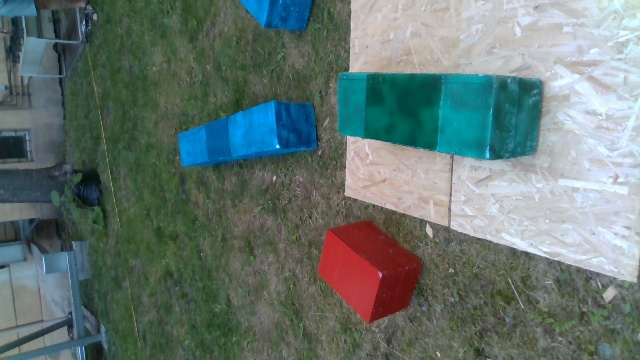
\includegraphics[width=\textwidth]{1.1}
    \caption{An example of scene taken from UAV with cuboid objects of different colors and shape}
    \label{fig:1-1}
\end{figure}

The task is originated from The Mohamed Bin Zayed International Robotics Challenge 2020 (MBZIRC 2020). Cuboid blocks are made of lightweight foam material. After detection, the objects are supposed to be taken by Unmanned Aerial Vehicle (UAV) using magnet holder and to be placed on a wall in specific pattern based on color and shape. For transportation purpose, the cuboid objects have also a metal plate painted with the same color on top of it. In real data-set the color of metal plate has slightly different color that introduces problems in object detection. 

UAV is equipped with Intel RealSense D435 camera (Fig.\ref{fig:d435}). The device integrates color image camera with set output 640x360 pixels (width x height) and depth image camera with set output 848x480 pixels. Such equipment allows different algorithms for object detection using color and depth images only as well as fused solution for both. The fusion of the algorithms is supposed to increase the quality and robustness of the detection.

\begin{figure}[htpb]
    \centering
    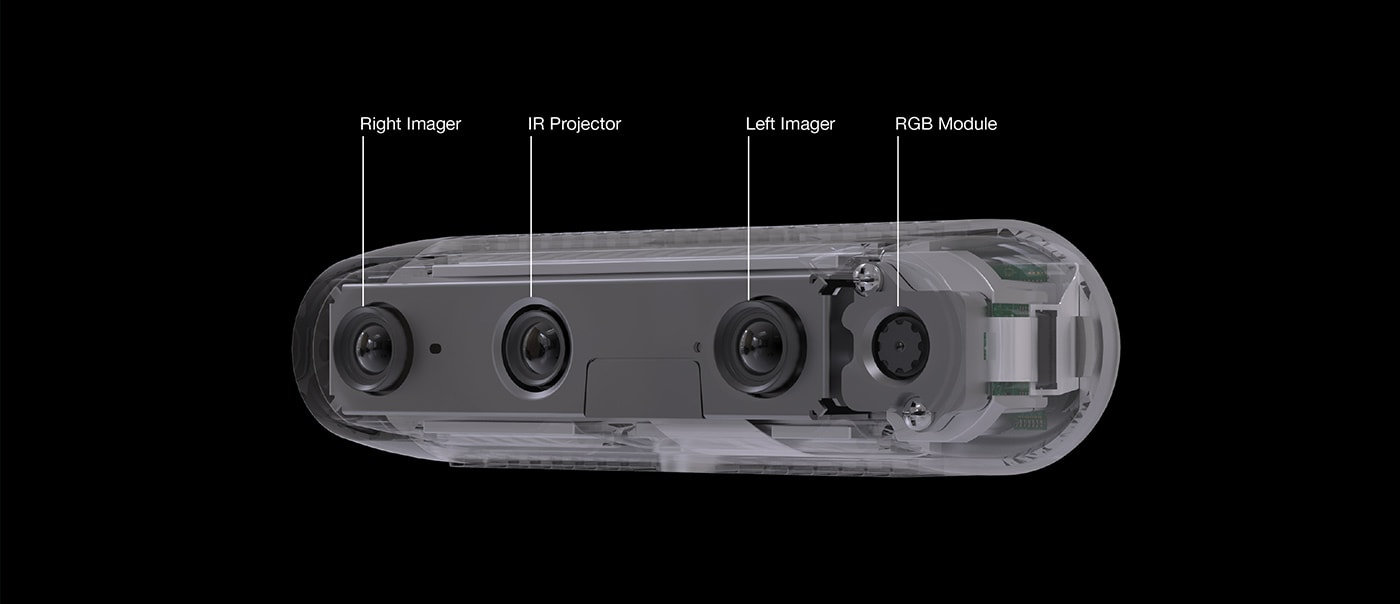
\includegraphics[width=\textwidth]{d435_camera_modules.jpg}
    \caption{Intel RealSense D435 camera. Source \cite{intel}}
    \label{fig:d435}
\end{figure}

Depth image is represented as depth map. Unlike to a color image, where pixel value represents color and its intensity, in a depth image pixel value itself represents the distance. Taking this into account, we can treat the depth image as a grid of distances. Conversion from pixel value to a distance value depends on camera setting. 
The depth is computed from stereo pair of infrared cameras with $50$~mm distance between cameras.
It's possible to reduce sensitivity and accuracy in a sake of maximum distance estimation. However, it should be noticed, that distance measurement is limited by 10 meters and suffer from noise on large distances, maximum value on image means that distance is out of measurement range. There is no a standard way to visualize a depth image, however an example of one of possible representations is shown on Fig.\ref{fig:1-3}, where brighter color means larger distance.

\begin{figure}[htpb]
    \centering
    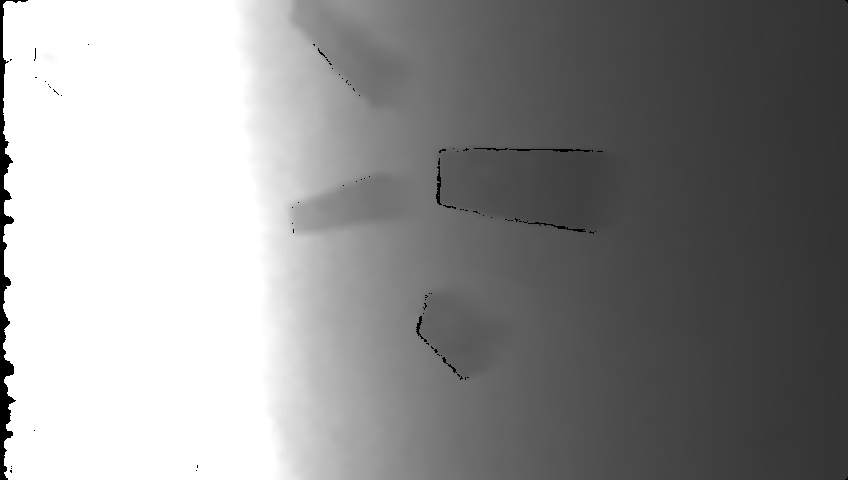
\includegraphics[width=\textwidth]{depth_example.jpg}
    \caption{An example of depth image representation}
    \label{fig:1-3}
\end{figure}

A depth image could be also converted to a point cloud. A point cloud is a form of representation of a scene in a 3D. As it led from the tittle, point cloud is a set of points distributed in the space, each of them has at least \{x, y, z\} coordinates, but it could have more properties (e.g. color). The example of a point cloud is shown on Fig.\ref{fig:1-4}.

To work with a point clouds, libraries, such as PCL (Point Cloud Library), could offer various built-in features to speed up the development process. The PCL is an open source library, distributed under BSD license and being developed by Willow Garage from March 2010. The library is designed for 3D geometry processing and three-dimensional computer vision algorithms. The library is supported by ROS and could be used for processing of point-based data taken from an depth camera, LIDAR etc.

\begin{figure}[htpb]
    \centering
    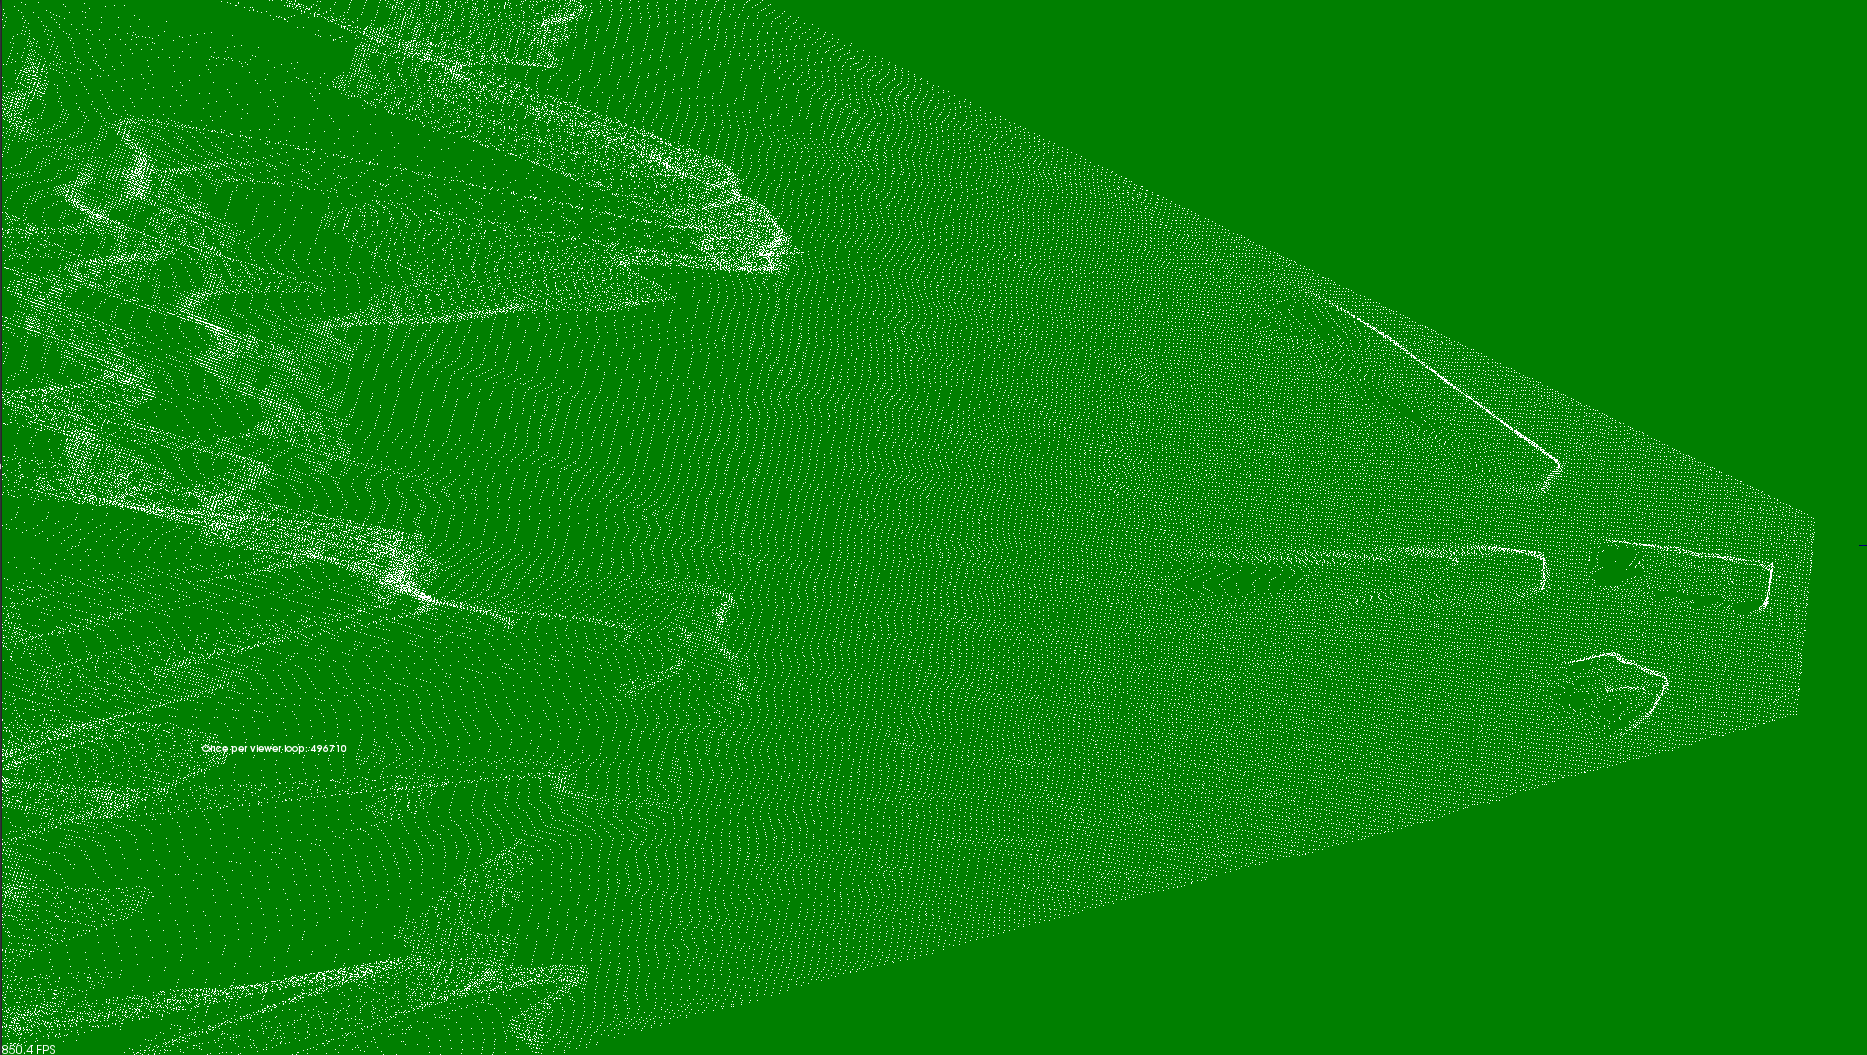
\includegraphics[width=\textwidth]{point_cloud_2.png}
    \caption{An example of a point cloud built from a depth image}
    \label{fig:1-4}
\end{figure}

ROS, which stands for Robot Operating System, is robotic middleware that's widely used in mobile robotics domain. In fact ROS is not an Operating System from a traditional point of view and it needs to be installed in Linux, MacOS (experimental) or Windows (experimental). Nevertheless, it gives capabilities which are common for any operating system. Such capabilities are hardware abstraction, typical low-level device control, threading (in form of nodes), message passing interface for nodes communication, package management. ROS started in Stanford University as a work of PhD students Eric Berger and Keenan Wyrobek. In 2007 they were invited to join Willow Garage and proceed the work under ROS.

Color image processing in this work has been mainly done using OpenCV library. OpenCV (Open Source Computer Vision Library), distributed under BSD license, is originally developed by Intel Research and contributed by Intel Russia and Intel's Performance Library Team. It was later supported by Willow Garage and integrated into ROS environment. The library is written in C/C++ programming languages and designed for Real Time Computer Vision tasks. Started in 1999, it was first released to public in 2000 during the IEEE Conference on Computer Vision and Pattern Recognition, and still actively evolves. OpenCV offers various algorithms for color image processing as well as machine learning tools, what makes it valuable among mobile robotics research groups. It also supports CUDA and OpenCL, what is important for usage in embedded domain.

The libraries provide detailed tutorials, which were actively used during the experiments.



\chapter{Methods of Detection for Color Image}
\section{Color Segmentation}

An algorithm based on color segmentation is the most intuitive and, as it resulted, the fastest in terms of computational speed approach for color object detection. Since all the objects for the search in the scene are of three different colors, we, as humans, could easily differentiate them in terms of color. The color segmentation algorithm is based on assessing of every image pixel color value and its comparison with some limits (or ranges). Ranges are taken as lower and upper limits in a color space. The limit values depend on color model chosen to represent an image, it's guided by color representation in a space, but exact values are found empirically. If the pixel is inside a range, it's marked as taken (i.e. set to logical True), or not taken otherwise (logical False). One of the output image representation could be a binary image, that uses only two colors - black for False and white for True. Taking into account this representation method, we can segment image on colors and get the output as shown on Fig.\ref{fig:2-1}.

\begin{figure}[htbp]
     \centering
     \begin{subfigure}{0.475\textwidth}
         \centering
         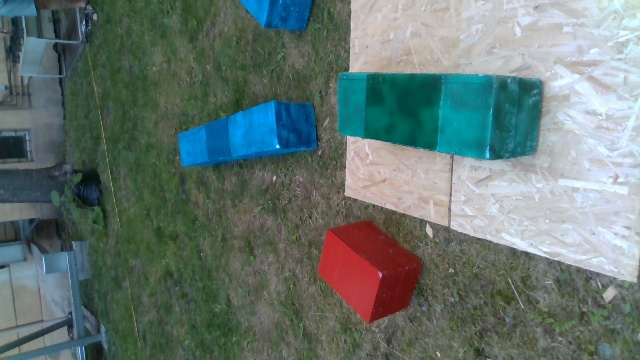
\includegraphics[width=\textwidth]{1.1.jpg}
         \caption{original scene}
         \label{fig:2-1-a}
     \end{subfigure}
     \hfill
     \begin{subfigure}{0.475\textwidth}
         \centering
         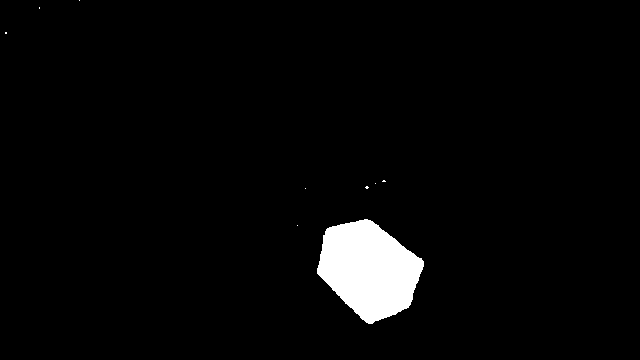
\includegraphics[width=\textwidth]{red_segmented.png}
         \caption{binary image for color segmented scene (red)}
         \label{fig:2-1-b}
     \end{subfigure}

        \caption{Example of color segmentation for red color}
        \label{fig:2-1}
\end{figure}

The color segmentation defines only potential regions, where such objects could be found, but it doesn't guarantee to detect only the objects of interest. Terrains and ground that are in range of color segmentation filters could be a cause of false positive detection. Typical examples of such issue could be grass that is usually close to green color or metal constructions which could be marked by blue color filter. Such false positive detected regions should be filtered out.

Another topic to consider is illumination. We need the color segmentation algorithm to include the range of all possible colors and tones that particular object could have in a scene with a different light source's intensities applied. Moreover, the metal plate, which is placed on top of every cuboid for transportation purpose, has different reflective properties. Hence, it makes the color range to be much wider that's needed for one scene. A broad range would yield higher number of interest regions that should be somehow processed and filtered after.

Intersection of color ranges could be also an issue. In case of a broad color range for proper object detection in a scene with different illuminations, we could observe that ranges for neighboring colors could have an intersection and therefore color segmentation output could have ovelapped regions. As an example, it's possible to face this problem for green and blue colors in HSV color space. Any such intersection could result a false positive detection.


\subsection{Color Models}
From physical point of view, pixel value is an amplified charge that caused by reflected light and collected in photosensitive element of an image sensor during exposure time. Photosensitive elements are stored in two dimensional image sensor array. In the digital domain black and white images, particularly grayscale images, could be stored as a digital 2D array, what reflects camera structure, where every pixel value defines intensity of light in a particular point. Maximal value corresponds to highest intensity, i.e. white color, zero intensity means "no light" or black color. Tones, visualised as shades of gray, are represented as values between minimum and maximum. 

\begin{figure}[htbp]
     \centering
     \begin{subfigure}{0.475\textwidth}
         \centering
         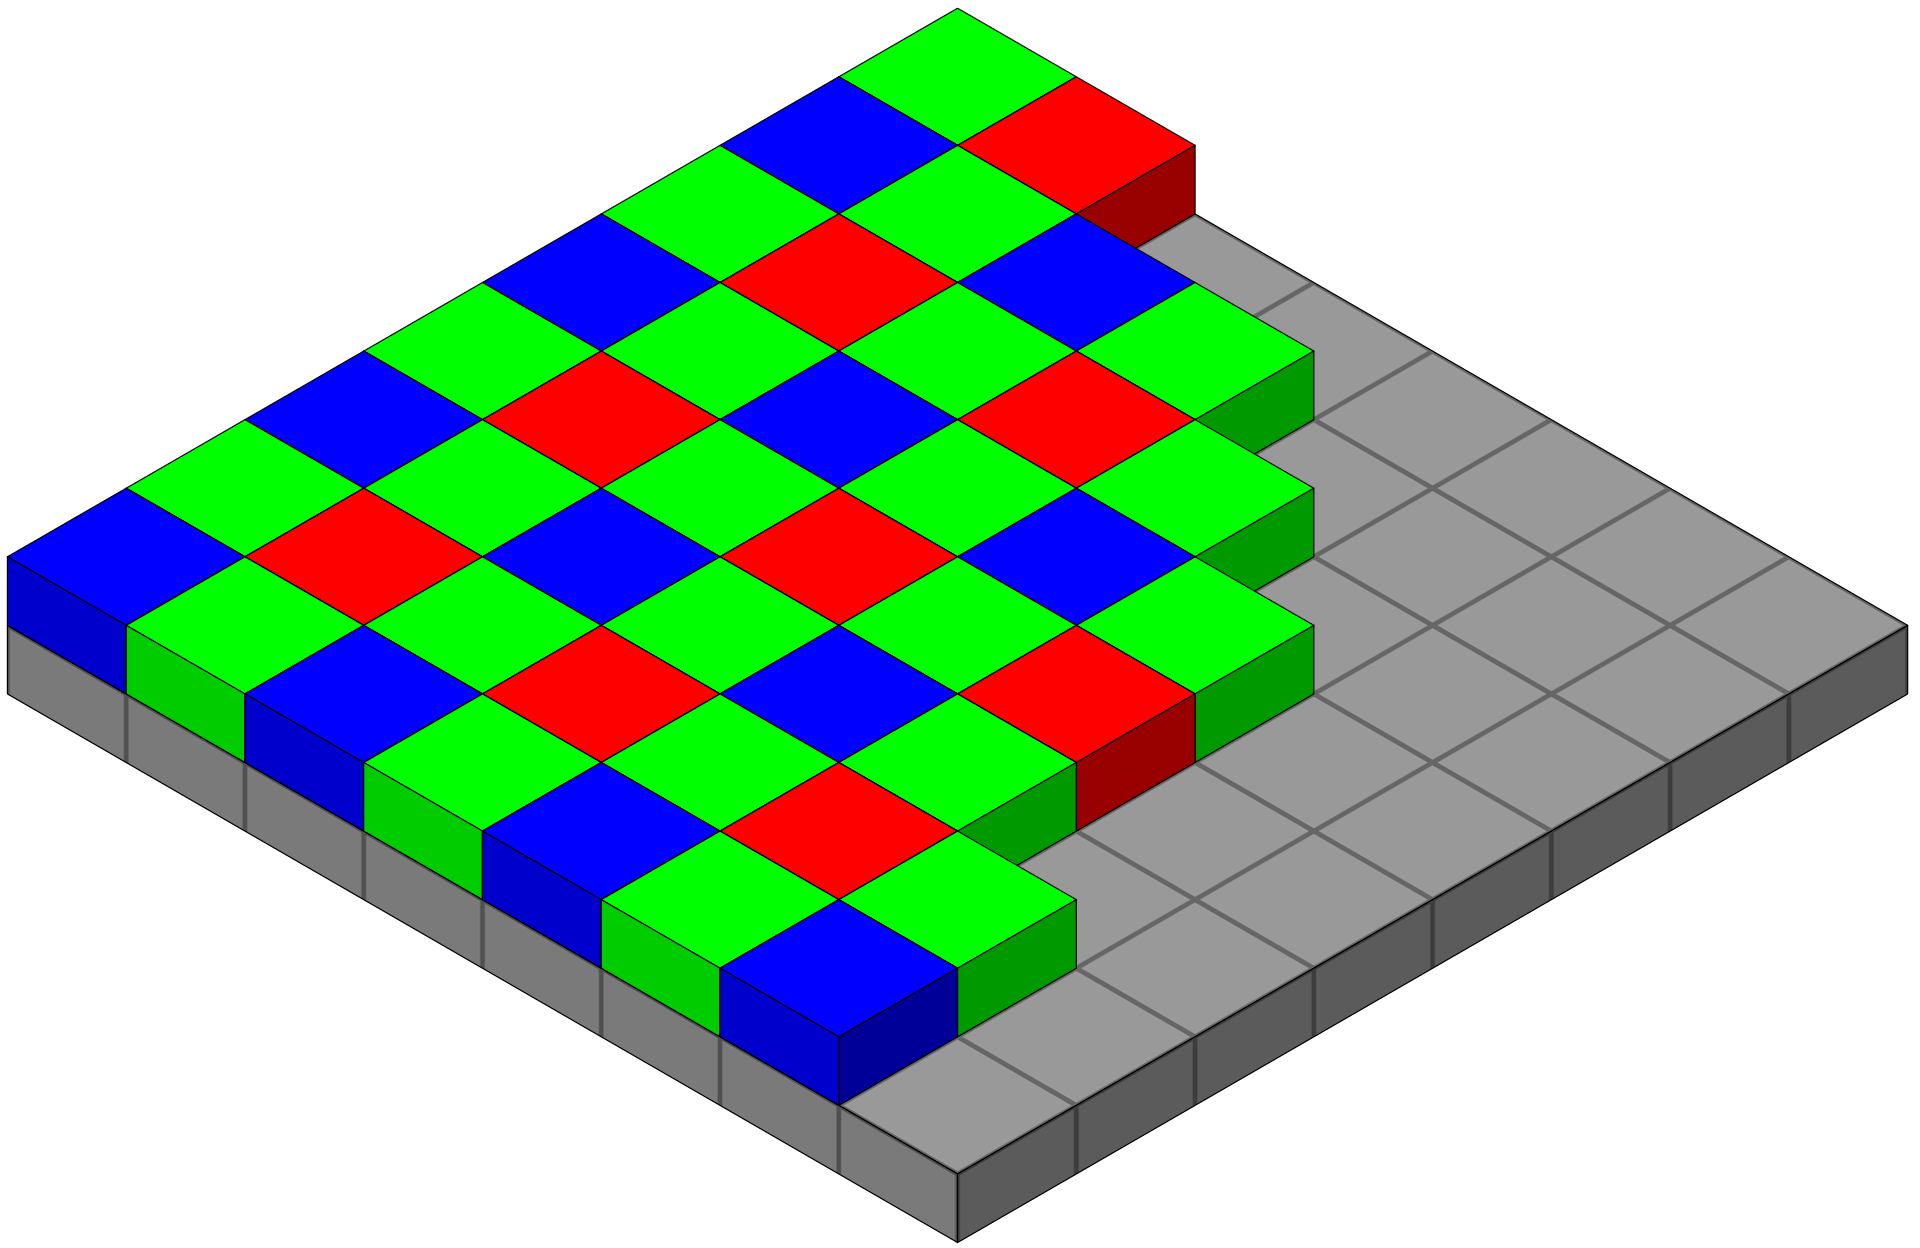
\includegraphics[width=\textwidth]{Bayer_pattern_on_sensor.svg.png}
         \caption{Bayer pattern. Image source\cite{bayerpattern}}
         \label{fig:2-2-a}
     \end{subfigure}
     \hfill
     \begin{subfigure}{0.475\textwidth}
         \centering
         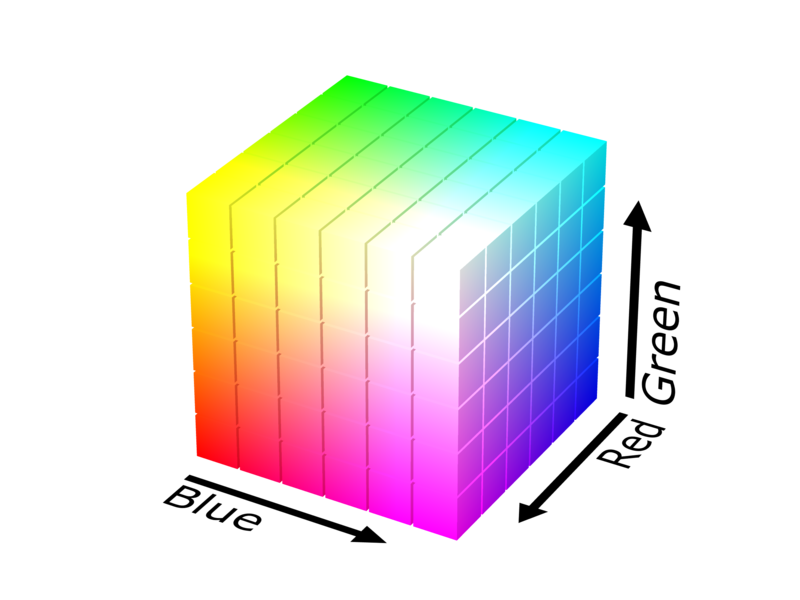
\includegraphics[width=\textwidth]{RGB_color_solid_cube.png}
         \caption{RGB color model. Image source\cite{rgbcolormodel}}
         \label{fig 2-2-b}
     \end{subfigure}

        \caption{Bayer pattern and RGB color model}
        \label{fig: 2-2}
\end{figure}

To create a color image, slightly more sophisticated method is used - to initial image sensor manufacturer applies a color filter, which is able to pass only the light inside specific range of wavelengths - wavelengths that correspond either to red, green or blue colors. Such filters are applied on an image sensor array in the Bayer pattern - Fig.\ref{fig:2-2-a}. Using this approach every pixel can store information only about one color, however it's possible to interpolate its neighbours for two other colors and get an averaged value to complete color information. In this case pixel color is defined by combination of intensities of red, green and blue colors. The color model is named RGB and it's currently the most used model today.

In the RGB model white color corresponds to the maximum for all three channels - red, green and blue. Black color - minimum for all the three. Examples for the illustration different shades of red color are shown on Fig.\ref{fig: rgb-example}.

\begin{figure}[htbp]
     \centering
     \begin{subfigure}{0.3\textwidth}
         \centering
         
\includegraphics[width=\textwidth]{100-50-50.png}
         \caption{R:100, G:50, B:50}
         \label{fig: rgb a}
     \end{subfigure}
     \hfill
     \begin{subfigure}{0.3\textwidth}
         \centering
         
\includegraphics[width=\textwidth]{250-50-50.png}
         \caption{R:250, G:50, B:50}
         \label{fig: rgb b}
     \end{subfigure}
          \hfill
     \begin{subfigure}{0.3\textwidth}
         \centering
         
\includegraphics[width=\textwidth]{250-200-200.png}
         \caption{R:250, G:200, B:200}
         \label{fig: rgb c}
     \end{subfigure}


        \caption{Example of different colors in RGB color range}
        \label{fig: rgb-example}
\end{figure}


The RGB model is not the best for color segmentation, because it doesn't separate brightness, \emph{luma}, from color information, \emph{chroma} and it could be a difficult to define a linear range in such color space for segmentation purpose. Taking this into account, we can use HSV model, which stands for Hue, Saturation, Value. The model is shown on Fig.\ref{fig:2-3}. The color information, Hue, is placed in a circular form, so it's possible to select a color for a range by the Hue parameter. Saturation defines color saturation - from white to clear color, value - amount of brightness from black to white. Color range in HSV could be visualised as a radial slice.

\begin{figure}[htbp]
    \centering
    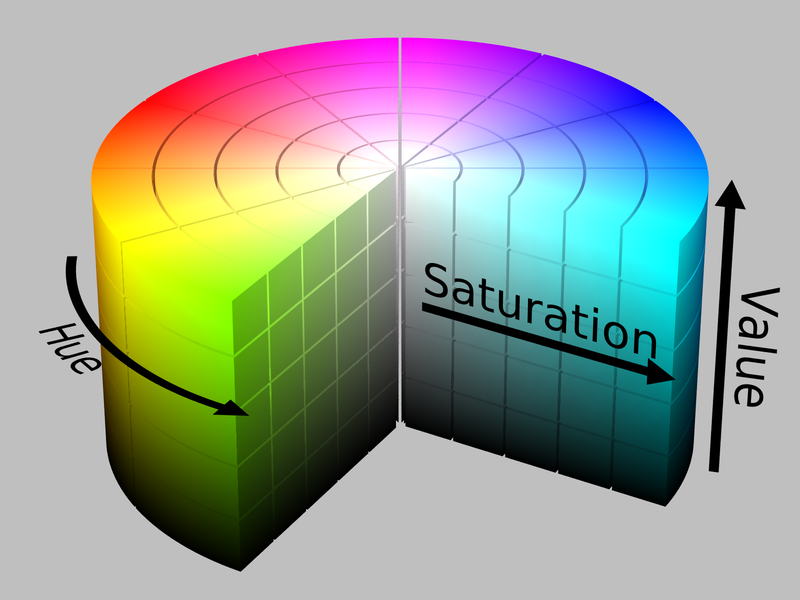
\includegraphics[width=0.75\textwidth]{800px-HSV_color_solid_cylinder_saturation_gray.png}
    \caption{HSV color model. Source \cite{hsvcolormodel}}
    \label{fig:2-3}
\end{figure}

To convert \{R, G, B\} color information into \{H, S, V\} following sequence should be applied. First, RGB values should be unscaled by division on maximum value in the scale (e.g. \emph {scale} = 255 for 8-bit color depth per channel image). Then maximal color value $c_{max}$, minimal $c_{min}$ and their difference $c_{diff}$ should be found. Once it has been obtained, Hue \emph{H}, Saturation \emph{S} and Value \emph{V} could be calculated. The final result should be scaled, typical value for $scale_H$ is 60 or 30 (that represent hue from 0-360, or 0-180 respectively), $scale_S=255$, $scale_V=255$.

\[ R' = \frac{R}{scale},\ \ G' = \frac{G}{scale},\ \ B' = \frac{B}{scale} \]

\[ c_{max} = max(R', G', B') \]
\[ c_{min} = min(R', G', B') \]
\[ c_{diff} = cmax - cmin \]

\[
    H= 
\begin{cases}
    0,& \text{if } c_{diff} = 0\\
    scale_H \cdot (\frac{G' - B'}{c_{diff}} \bmod 6), & \text{if } c_{max} = R'\\
    scale_H \cdot (\frac{B' - R'}{c_{diff}} + 2), & \text{if } c_{max} = G'\\
    scale_H \cdot (\frac{R' - G'}{c_{diff}} + 4), & \text{if } c_{max} = B'\\
\end{cases}
\]

\[
    S= 
\begin{cases}
    0,& \text{if } c_{max} = 0\\
    scale_S \cdot \frac{c_{diff}}{c_{max}}  ,              & \text{otherwise}
\end{cases}
\]

\[ V = scale_V \cdot c_{max}  \]

\subsection{HSV Color Range}
For correct HSV color range estimation, an additional HSV tool in form of Python script was developed (and attached as supportive file). The idea of the tool is to let an user to select area on a picture as an input, transform the image into HSV color space and build an histogram for Hue, Saturation and Value parameters in the selected crop area. An example of the tool output is shown in Fig.\ref{fig: hsv-tool}.
\begin{figure}[htbp]
     \centering
     \begin{subfigure}{0.475\textwidth}
         \centering
         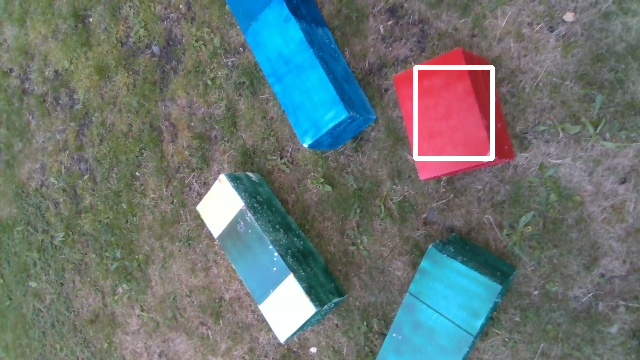
\includegraphics[width=\textwidth]{HSV_all.png}
         \caption{Initial image with user input}
         \label{fig: hsv a}
     \end{subfigure}
     \hfill
     \begin{subfigure}{0.475\textwidth}
         \centering
         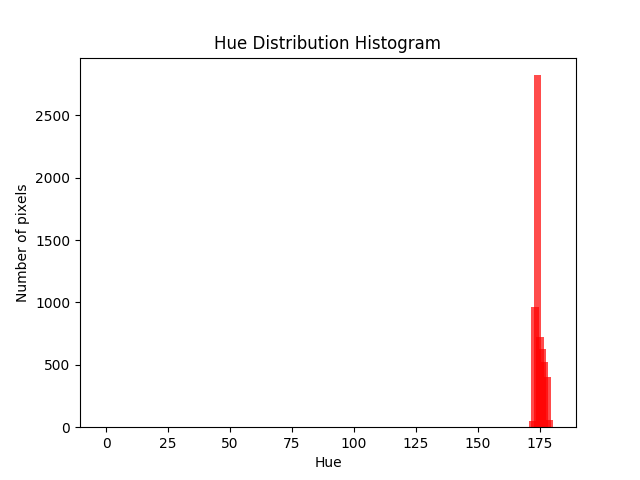
\includegraphics[width=\textwidth]{HSV_H.png}
         \caption{Histogram of Hue distribution }
         \label{fig: hsv b}
     \end{subfigure}
          \hfill
     \begin{subfigure}{0.475\textwidth}
         \centering
         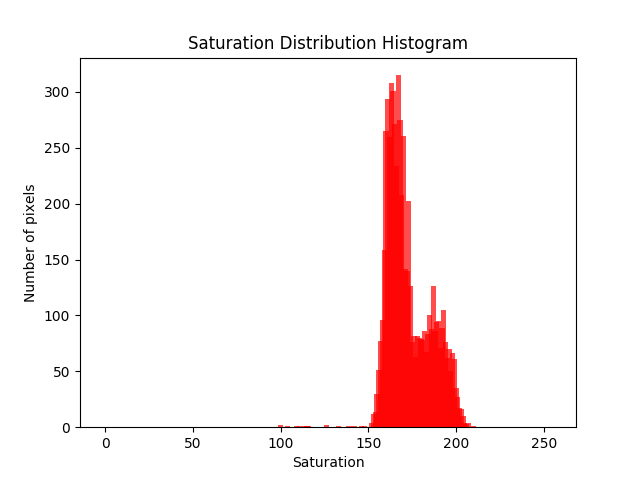
\includegraphics[width=\textwidth]{HSV_S.png}
         \caption{Histogram of Saturation distribution into selected area}
         \label{fig: hsv c}
     \end{subfigure}
          \hfill
     \begin{subfigure}{0.475\textwidth}
         \centering
         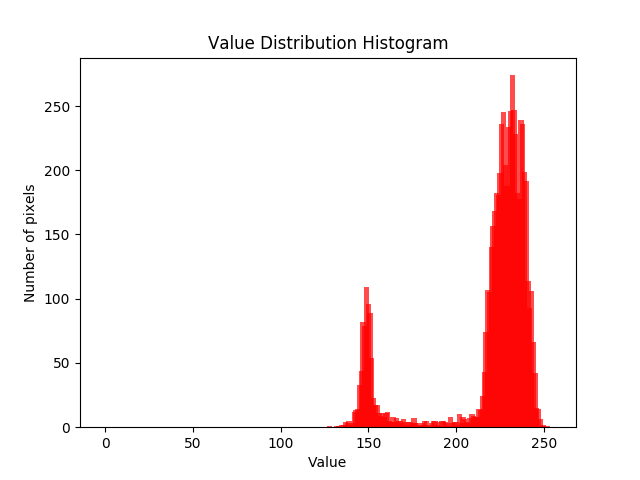
\includegraphics[width=\textwidth]{HSV_V.png}
         \caption{Histogram of Value distribution into selected area}
         \label{fig: hsv d}
     \end{subfigure}

        \caption{HSV tool usage example}
        \label{fig: hsv-tool}
\end{figure}

The tool is used to define ranges for correct object detection in given dataset. The dataset is made in form of ROS bag and was recorded by MRS team during the challenge preparation. At the first step, user should manually define ranges based on selected areas. When initial ranges are defined, they can be checked using the same tool and confirmed in semi-automated mode. The tool can use given range and visualise found region in series. User should accept or reject given contour, in case the object is taken, the tool memorises its HSV distribution to create the final HSV ranges. It was found useful, to set the initial ranges wider than it should be, so it guarantees complete object recall. False positives could be rejected during user's visual check, so the resulting distribution would still have complete and correct HSV ranges. The result of such tool are shown on Fig.\ref{fig:tot_H}, \ref{fig:tot_S} and \ref{fig:tot_V}.

\begin{figure}[htbp]
    \centering
    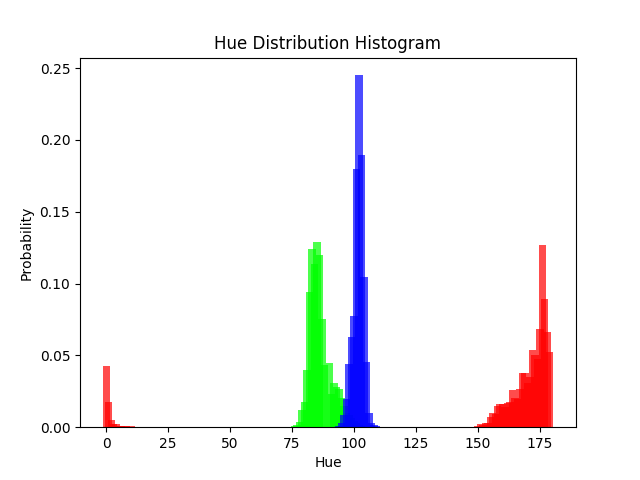
\includegraphics[width=\textwidth]{HSV_tot_H.png}
    \caption{Histogram of Hue distribution for cuboids}
    \label{fig:tot_H}
\end{figure}

\begin{figure}[htbp]
    \centering
    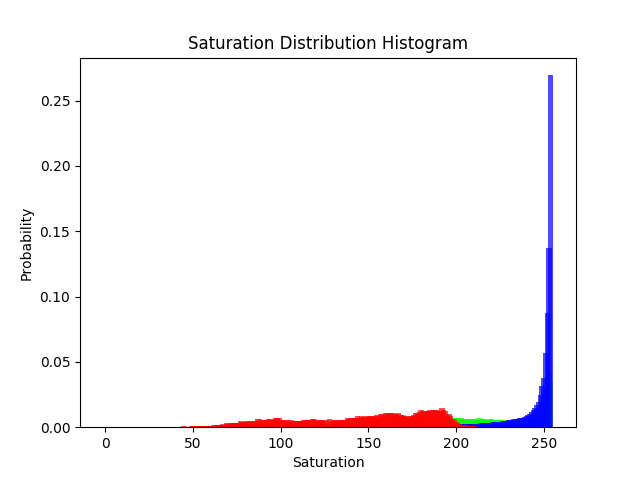
\includegraphics[width=\textwidth]{HSV_tot_S.png}
    \caption{Histogram of Saturation distribution for cuboids}
    \label{fig:tot_S}
\end{figure}

\begin{figure}[htbp]
    \centering
    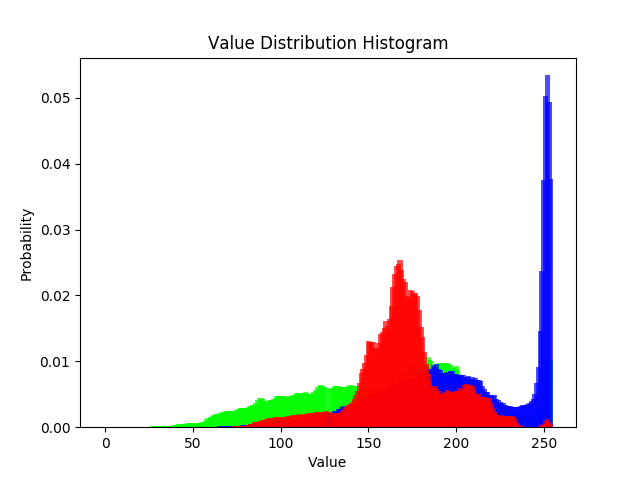
\includegraphics[width=\textwidth]{HSV_tot_V.png}
    \caption{Histogram of Value distribution for cuboids}
    \label{fig:tot_V}
\end{figure}

Based on obtained color ranges, it's obvious that ranges of neighbouring colors have an intersection. It makes the final algorithm to filter false positives in case full ranges are taken or to select unique ranges with no intersections, but it would require additional actions to find pixels of missed color range and get the full object area. 



\subsection{Algorithm based on HSV Color Range} \label{csa}

Algorithm takes as input image and pre-defined color ranges. To perform color segmentation, input image should be converted into HSV color space. Then image is processed separately for every color. Algorithm takes color range for specific color and creates binary image, where pixels inside the range are marked as True and False otherwise. It may be possible, that several objects of the same color are present on image as well as false positive objects. 
To filter false positive objects, algorithm checks found area and compare it with some threshold. Too small areas are rejected. Another property is number of lines needed to create an approximate contour of the area. It was found, that area, which contour consists of high number of lines, more likely to represent a false positive (as grass for green color).

\begin{algorithm}
\caption{Color segmentation in HSV color range}\label{hsv}
\begin{algorithmic}[1]

\State $image \gets input\ image$
\State $color\_range[r,g,b] \gets HSV\ color\ ranges$
\Procedure{color\_segm}{$image,color\_range[r,g,b]$}
\State $result \gets \emptyset$
\State $hsv\_image \gets cv2.cvtColor(image, cv2.COLOR\_RGB2HSV)$
\For{each color in $color\_range$ }
\State $candidates \gets cv2.inRange(hsv\_image, color\_range[color])$
\For{each candidate in $candidates$ }
\State $if\ getArea(candidate) < area\_threshold:\ continue$
\State $polyline \gets getPolyline(candidate)$
\State $if\ len(polyline) > lines\_threshold:\ continue$
\State $result \gets candidate$
\EndFor
\EndFor
\EndProcedure

\end{algorithmic}
\end{algorithm}

The filtering helps to reject most of false positives, but it doesn't guarantee error free detection. Hence more sophisticated filtering techniques should be used and reviewed. Another topic to consider is neighbor color region overlap. One of such technique to reject overlapped areas could be region voting. Once algorithm collected all candidates, it can sort them in descending order in terms of region area. Then algorithm add candidates to final result, if and only if more than 90\% of candidate region is not occupied by any of previous regions. It was found, that in case of range intersection, wrong contours are always inside larger contours, so such filtering could help to reject overlapped regions.

\begin{algorithm}
\caption{Region voting for color segmentation}\label{reg-vote}
\begin{algorithmic}[1]
\State $result \gets \emptyset$
\State $dummy\_image \gets empty\_image(size=input\ image)$
\State $color\_range[r,g,b] \gets HSV\ color\ ranges$
\State $candidates \gets color\_segm(image,color\_range[r,g,b])$
\State $candidates \gets sort(candidates)$
\For{each candidate in $candidates$ }
\State $iff\ candidate \cup dummy\_image > area\_threshold:\ continue$
\State $dummy\_image[candidate] \gets 1$
\State $result \gets candidate$
\EndFor
\end{algorithmic}
\end{algorithm}

\begin{figure}[htbp]
     \centering
     \begin{subfigure}{0.475\textwidth}
         \centering
         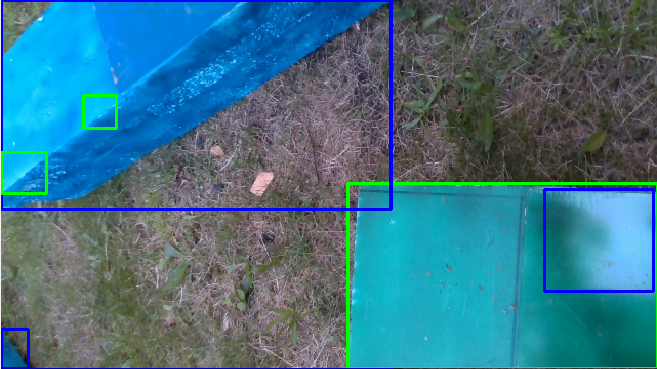
\includegraphics[width=\textwidth]{reg_vot_0.png}
         \caption{Initial region candidates}
         \label{fig: reg a}
     \end{subfigure}
     \hfill
     \begin{subfigure}{0.475\textwidth}
         \centering
         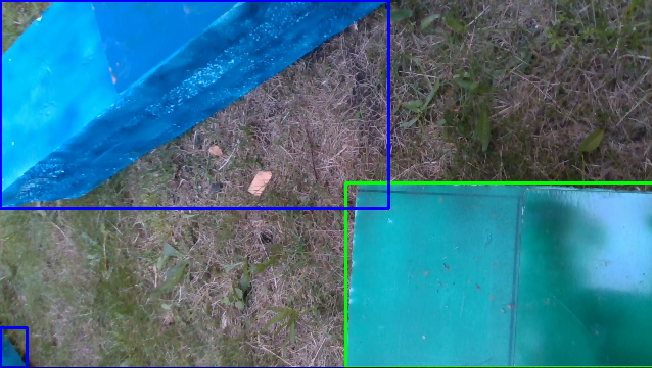
\includegraphics[width=\textwidth]{reg_vot_1.png}
         \caption{Candidates after region voting}
         \label{fig: reg b}
     \end{subfigure}

        \caption{Region Voting Filter}
        \label{fig: reg-v}
\end{figure}

It's supposed to be also improved by time memory and optical flow. Every selected region could have probability of some color based on all previous detection. Region memory should be shifted by optical flow information. It gives region voting algorithm an advantage in form of filtering of regions with low probability in order to reject region overlap.


\section{Algorithm based on Graph Cut (GrabCut)}

The segmentation based on color range is simple and quick, but it suffer from range intersections, region overlap and excessive regions detected. One of possible improvement could be segmentation based on traversing through image as a graph. One of such approaches - interactive foreground extraction - is using GrabCut algorithm.

The algorithm was introduced by Carsten Rother, Vladimir Kolmogorov and Andrew Blake from Microsoft Research Cambridge in their work \cite{grabuct}. It was presented as improvement for automatic segmentation algorithms such as Magic Wand from Adobe Photoshop 7 \cite{adobe}, Intelligent Scissors (a.k.a. Live Wire or Magnetic Lasso) \cite{intsci} and Graph Cut [Boykov and Jolly 2001; Greig et al. 1989] \cite{graphcut}.

The algorithm takes the image and rectangle-shaped user input, inside which the object is located. Anything outside the user input box will be treated as sure background. Then algorithm represents the image as graph and creates energy function. Every pixel is represented as graph node, and specific weight assigned to each edge, that connects nodes. %PS which nodes are connected? only 4 neighbour pixels? 
The weight is computed based on edge information or pixel similarity. If difference between two neighboring pixels (nodes) is large, the edge weight will be small. Then all the nodes should be assigned either to Background terminal T or Object terminal S in such way, that graph cut, which separates terminals, will have minimal total energy. Such cut will result the best segmentation. The principle is illustrated on Fig.\ref{fig:GrabCut}.


\begin{figure}[htbp]
    \centering
    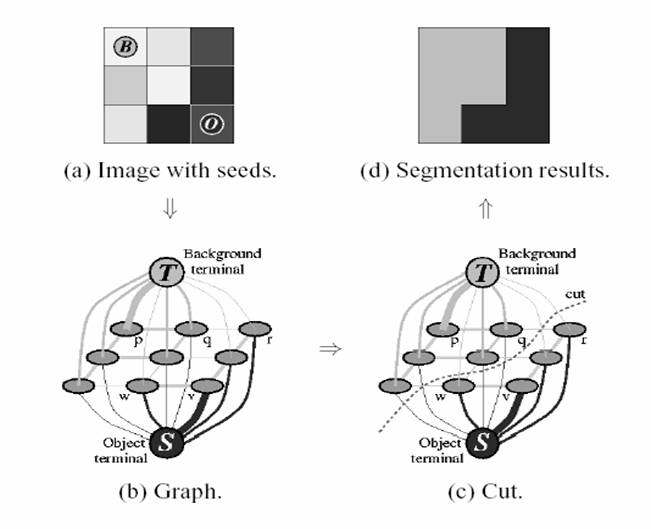
\includegraphics[width=\textwidth]{grabcut.jpg}
    \caption{Simplified illustration of GrabCut algorithm. Source \cite{grabcut_pic}}
    \label{fig:GrabCut}
\end{figure}

To use the algorithm, color segmentation with strictly unique ranges (i.e. no range intersection is allowed) is taken in order to obtain strong color regions, which will be then enlarged to compensate lost parts because of insufficient color range and passed to GrabCut algorithm. The result for one region of blue cuboid color range is shown on Fig.\ref{fig: gc-ex} as an example.

\begin{figure}[htbp]
     \centering
     \begin{subfigure}{0.475\textwidth}
         \centering
         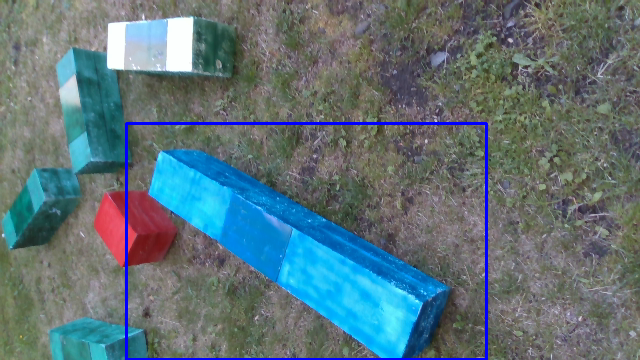
\includegraphics[width=\textwidth]{GrabCut_init.png}
         \caption{Initial image with user input}
         \label{fig: gc-ex a}
     \end{subfigure}
     \hfill
     \begin{subfigure}{0.475\textwidth}
         \centering
         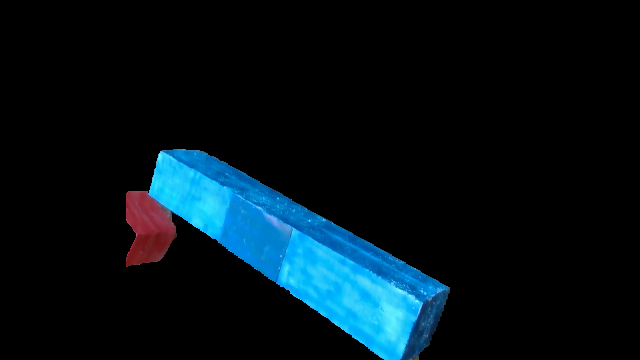
\includegraphics[width=\textwidth]{GrabCut_result.png}
         \caption{GrabCut algorithm output}
         \label{fig gc-ex b}
     \end{subfigure}

        \caption{GrabCut usage example}
        \label{fig: gc-ex}
\end{figure}

As you can see at Fig.\ref{fig: gc-ex}, algorithm can detect background accurately, however cuboid of another color is also selected as foreground. In such case, algorithm is deemed to accept clarifications in terms of additional user input, which could be foreground and background. For such purpose, we can use output image and do color segmentation for other colors. Any detected cuboid of other color will be processed to GrabCut algorithm as sure background and algorithm will be called again. The final output is shown on Fig.\ref{fig:GrabCut_final}.

\begin{figure}[htbp]
    \centering
    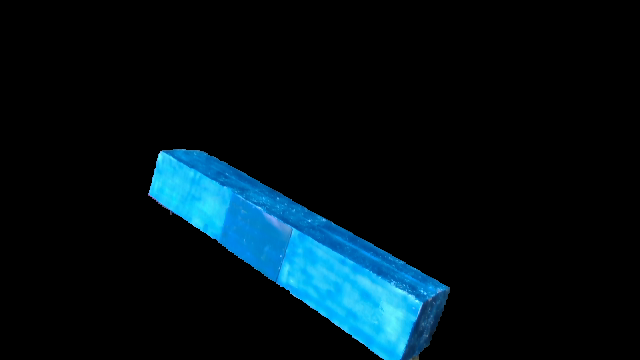
\includegraphics[width=12cm]{GrabCut_result_updated.png}
    \caption{Updated image after background clarification for GrabCut algorithm}
    \label{fig:GrabCut_final}
\end{figure}


\begin{algorithm}
\caption{Cuboid object detection with GrabCut algorithm}\label{grabcut}
\begin{algorithmic}[1]
\State $result \gets \emptyset$
\State $image \gets input\ image$
\State $color\_range[r,g,b] \gets HSV\ color\ ranges$
\State $regions \gets color\_segm(image, color\_range[r,g,b])$
\For{each region in $regions$ }
\State $color = region\ color$
\State $mask = empty\ mask$
\State $bbox = enlarged\ region\ bbox(region, enl\_coeff)$
\State $mask = cv2.GrabCut(image, bbox, mask)$
\State $mask\_new = color\_segm(image[mask != 0], color\_range[\lnot color])$
\State $mask = mask \oplus mask\_new$
\State $mask = cv2.GrabCut(image, bbox, mask)$
\State $result \gets image[mask != 0]$
\EndFor

\end{algorithmic}
\end{algorithm}



Complete algorithm is described in the Algorithm \ref{grabcut} section. As the result, proposed solution could accurately segment cuboid objects in the most of cases. Main disadvantage of such approach is computational speed. The algorithm is far from real time and it takes more than 4 seconds for single region processing on Intel Core i7-2630QM processor @ 2.00 GHz.

\section{Algorithm based on a Search of Closed Loop}
Another graph method for object segmentation is a closed loop search based on edge information. The method is an attempt to improve computation speed of GrabCut algorithm.

\begin{algorithm}
\caption{Cuboid object detection with closed loop search algorithm}\label{clloop}
\begin{algorithmic}[1]
\State $result \gets \emptyset$
\State $image \gets input\ image$
\State $I_X, I_Y \gets gradient(image)$
\State $sobel \gets \sqrt{I_X^2 + I_Y^2}$
\State $bin\_image \gets binary\_threshold(sobel, threshold)$
\State $diluted \gets dilution(bin\_image)$
\State $skel \gets skeleton(diluted)$

\State $color\_range[r,g,b] \gets HSV\ color\ ranges$
\State $regions \gets color\_segm(image, color\_range[r,g,b])$
\For{each region in $regions$ }

\State $corner\_pixel \gets find\_corner\_pixel(region)$
\For{each pixel around $corner\_pixel$ }
\State $if\ (pixel \neq edge\_pixel): continue$
\For{each $edge\_pixel$ }
\State $closed\_loop \gets search\_for\_closed\_loop(skel)$

\For{each $closed\_loop$ }
\State $Q = calc\_quality(closed\_loop)$
\State $if\ Q > Q\_THRESHOLD,\ result \gets closed\_loop $
\EndFor
\EndFor
\EndFor
\EndFor

\end{algorithmic}
\end{algorithm}


As it stated in the algorithm section, the method is based on Sobel filter \cite{sob}, which computes image gradients $I_x$, $I_y$ (in x and y directions respectively) and produces resulting gradient as $\sqrt{I_X^2 + I_Y^2}$. The illustration of sobel filtering is shown on Fig.\ref{fig:2-7}.

\begin{figure}[htbp]
     \centering
     \begin{subfigure}{0.475\textwidth}
         \centering
         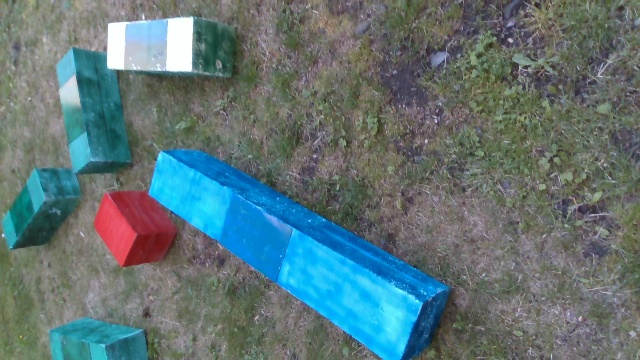
\includegraphics[width=\textwidth]{orig_cl.jpg}
         \caption{original scene}
         \label{fig:sob-a}
     \end{subfigure}
     \hfill
     \begin{subfigure}{0.475\textwidth}
         \centering
         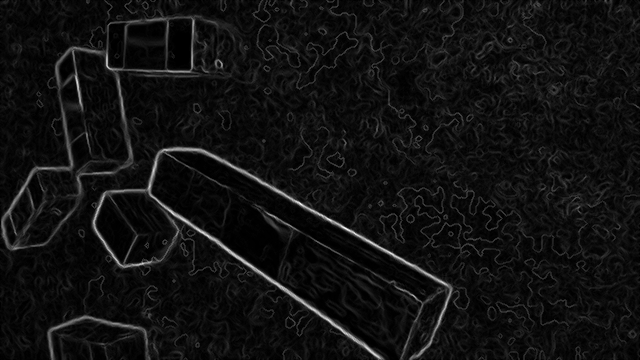
\includegraphics[width=\textwidth]{sobel.png}
         \caption{Sobel operator applied to original image}
         \label{fig:sob-b}
     \end{subfigure}

        \caption{Example of sobel filtering}
        \label{fig:2-7}
\end{figure}

The next step is threshold filter which will result a binary image. The threshold should be set small enough so even weak gradients will be surely taken. The binary image is then processed in order to obtain a skeleton image. The result of those operations are shown on Fig.\ref{fig:2-8}. 

\begin{figure}[htbp]
     \centering
     \begin{subfigure}{0.475\textwidth}
         \centering
         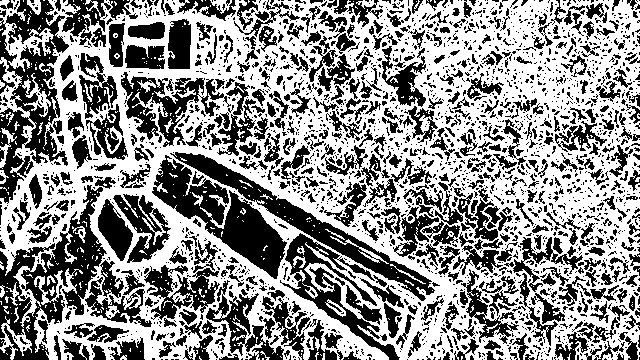
\includegraphics[width=\textwidth]{bin.png}
         \caption{Binary image as output of threshold filter}
         \label{fig:bin}
     \end{subfigure}
     \hfill
     \begin{subfigure}{0.475\textwidth}
         \centering
         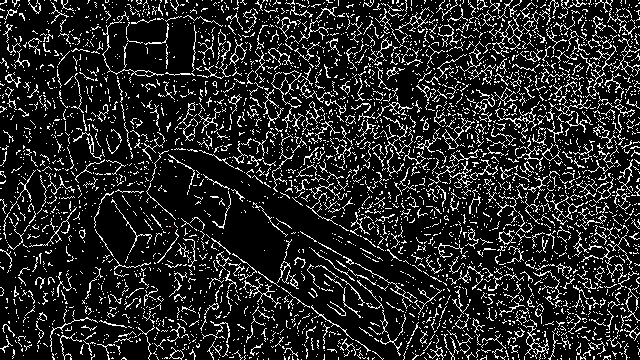
\includegraphics[width=\textwidth]{skel.png}
         \caption{Skeleton image}
         \label{fig:skel}
     \end{subfigure}

        \caption{Example of threshold filter and skeleton image}
        \label{fig:2-8}
\end{figure}

As the result skeleton image could be used for traversing through edges, i.e. white pixels, in order to find closed loops. Breadth-first search algorithm was used for the traversing and search in the proposed method. Regions, detected with color segmentation algorithm with unique ranges, could be used as initial region mask. Algorithm starts from a mask frontier pixel, i.e. front pixel that splits "1" and "0" zones of initial mask, and finds closest edge, i.e. white pixel, around segmented region and switches to search for a closed loops. When such loop is found, algorithm assess it in terms of closed loop quality as intersection of color segmented region and found closed loop area over color segmented region. The closed loop quality Q shows ratio of color region pixels inside the closed loop to total number of color region pixels. Therefore, value that close to 1 or above some threshold is a break condition for the search process.
\\

\[ Q = \frac{color\ region \cap closed\ loop}{color\ region} \]
\\

\begin{figure}[htbp]
    \centering
    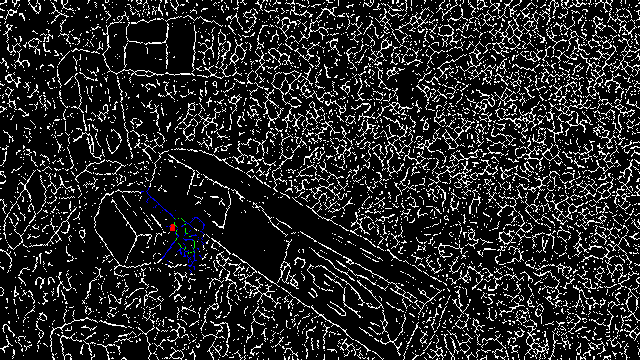
\includegraphics[width=\textwidth]{quality0.png}
    \caption{First found closed loop (Q = 0). Legend: red - original mask from color segmentation step, blue - checked contour, green - closed loop found}
    \label{fig:q0-cl}
\end{figure}


\begin{figure}[htbp]
    \centering
    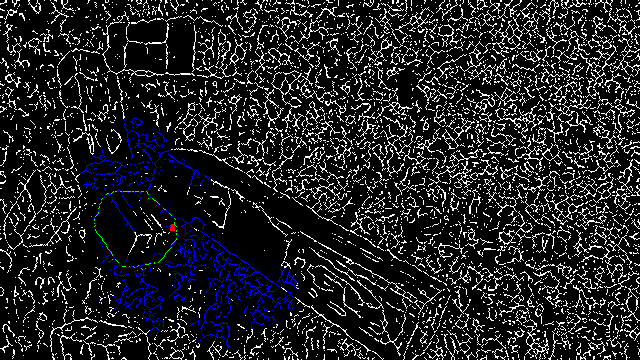
\includegraphics[width=\textwidth]{quality100.png}
    \caption{Closed loop with Q = 1.0. Legend: red - original mask from color segmentation step, blue - checked contour, green - closed loop found}
    \label{fig:q100-cl}
\end{figure}


Figures \ref{fig:q0-cl}, \ref{fig:q100-cl} and \ref{fig:gc-q} are examples of object detection based on closed loop search. Detection is performed against red color. Color segmentation mask with a strict color range is shown on Fig.\ref{fig:scm}. For illustration purpose the start pixels from the initial segmented mask are colored red. Algorithm explores pixel around the segmented mask and searches for the closest edge. When edge is found, algorithm traverse through all its neighbour until closed loop (cycle) is detected. Processed edges are highlighted by blue color, found loop - green. When the loop is found algorithm computes its quality and if it's above some threshold, it returns found contour or proceed the search otherwise. The first found loop is shown on Fig.\ref{fig:q0-cl}. The quality of such loop is low, as it seen on the figure, the loop is outside the block, so there will be no initial mask pixels inside the found loop corner. Algorithm proceed the search until loop on Fig.\ref{fig:q100-cl} is found. Based on initial and closed loop masks (Fig.\ref{fig:gc-q}), quality of the loop is equal to 1.0, thus it generates break condition and algorithm stores the loop into the result.



\begin{figure}[htbp]
     \centering
     \begin{subfigure}{0.475\textwidth}
         \centering
         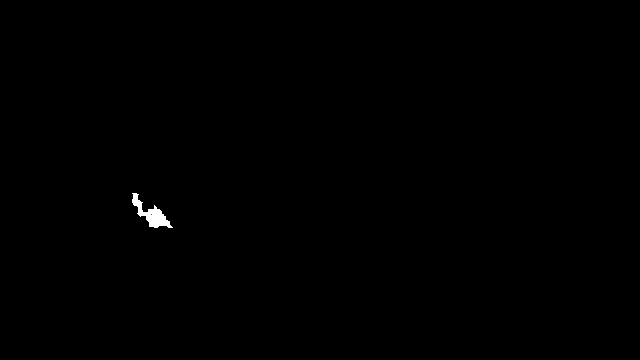
\includegraphics[width=\textwidth]{mask.png}
         \caption{Segmented color mask}
         \label{fig:scm}
     \end{subfigure}
     \hfill
     \begin{subfigure}{0.475\textwidth}
         \centering
         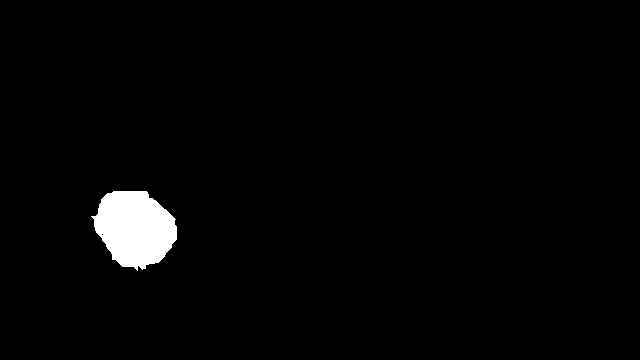
\includegraphics[width=\textwidth]{loop mask.png}
         \caption{Closed loop mask}
         \label{fig:clm}
     \end{subfigure}

        \caption{Example of closed loop search. Legend: red - original mask from color segmentation step, blue - checked contour, green - closed loop found}
        \label{fig:gc-q}
\end{figure}

The algorithm has several points to consider, one of them is that the algorithm is very sensitive to threshold values chosen for edge filtering, because it can yield to poor skeleton image. It may result, that proposed coefficients would be not correct for detection with another image sensor device or in different scene, and some edges would be missed. On the other hand, the low coefficients can lead to weak edges detection with multiple false closed loop detection.
In the first case it yields to huge gaps between the edges such that algorithm will not be able to accurately detect the loop or in second case, it could waste time on looping on textures around.

Another weak point of this algorithm is computational speed. Python implementation of this method was found to be slow for the graph task. Overall computational speed was a maximum among all the used approaches - the loop on Fig.\ref{fig:q100-cl} was found for more than 10 seconds on Intel Core i7-2630QM @ 2.00 GHz. It's supposed (but not implemented), that C or C++ implementation of the algorithm could have much better speed performance. Moreover, there is room for algorithmic improvements, one of them could be usage of heuristics in closed loop search in a way that edges that are closer to initial mask could be processed sooner, e.g. based on Manhattan or Euclidean distance from edge pixel being traversed to the color region. Such approach is inspired from A* algorithm \cite{astar} where it's used as an heuristic optimisation.

\section{Deep Learning and Convolutional Neural Networks}

Many tasks of Computer Vision today are being solved by Artificial Neural Networks. Solutions based on Neural Networks are state-of-the-art in many areas such as object detection and image recognition, semantic and instance segmentation, image colorization, style transfer and others.

The Neural Networks are computing systems inspired by biological neural networks, where its nodes, \emph{neurons}, are connected with other nodes in some system and can pass signal to these connected nodes. Nodes and connections typically have a weight, which is initialised to a random number and adjusted during training process. These weights are applied to signal passed by neurons and resulted signal is propagated to connected neurons. The Neural Network output usually comes from a non-linear activation function, e.g. sigmoid, hyperbolic tangent, Rectified Linear Unit and others. Meaning of the output could vary on architecture of the neural network and its task. In case of object detection it can be 1D array, where each value stands for confidence of object to be of particular class, or in case of image generation as style transfer it could be an image itself in form of array of three 2D outputs (for three color channels - RGB), where each value stands for output image pixel value. Convolutional Neural Networks are used to work with images. Convolution operation is applied to input image with a layer weights.

\begin{figure}[htbp]
    \centering
    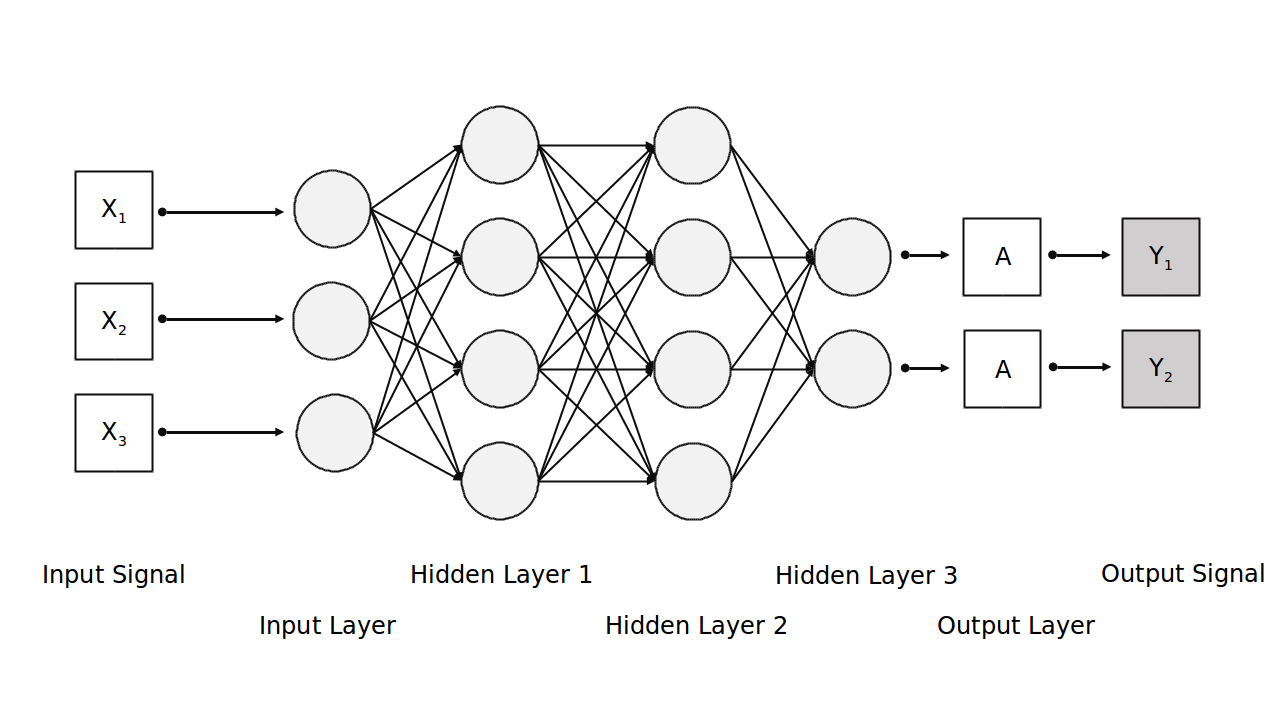
\includegraphics[width=\textwidth]{nn_arch.png}
    \caption{Neural Network Structure}
    \label{fig:nn}
\end{figure}

Two different methods based on Neural Networks are studied in this work - Holistically-Nested Edge Detection published by Saining Xie et al., 2015 \cite{hne} as way to improve closed loop search and object detection with instance segmentation YOLO v2 tiny published by Joseph Redmon et al., 2016 \cite{yolo}.

\subsection{Holistically-Nested Edge Detection}

Holistically-Nested Edge Detection based on Convolutional Neural Network is an algorithm to predict image edges. The work was published by Saining Xie and Zhuowen Tu in 2015 \cite{hne} and was aimed to solve fundamental problems of Computer Vision in terms of object boundaries and edge detection. Neural Network was designed in order to provide multi-scale and multi-level feature learning. It was trained on BSD500 and NYU Depth datasets and demostrated fast computation speed (0.4 seconds per image was committed by the authors). Pretrained network models are publicly available by authors, hence it can be used in OpenCV environment for the test.

\begin{figure}[htbp]
    \centering
    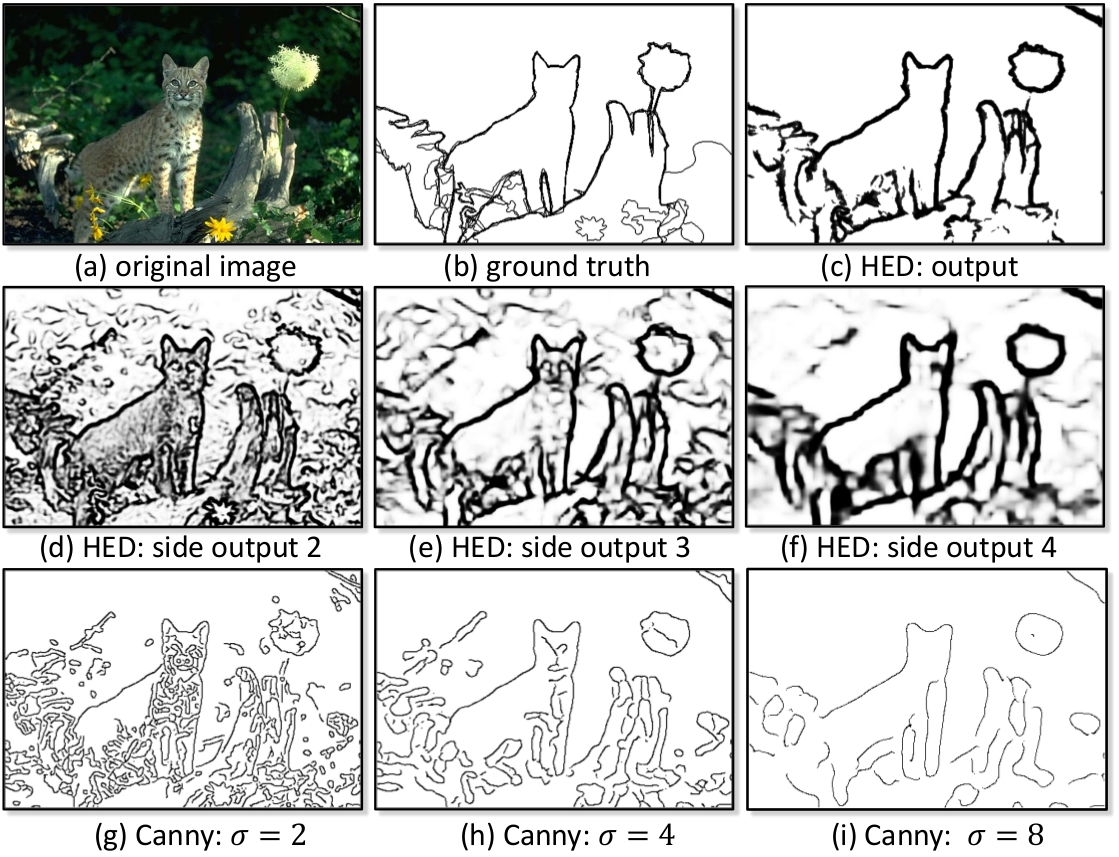
\includegraphics[width=\textwidth]{hne.png}
    \caption{Example of Holistically-Nested Edge Detection performance. Source \cite{hne}}
    \label{fig:hne-ex}
\end{figure}

\begin{figure}[htbp]
    \centering
    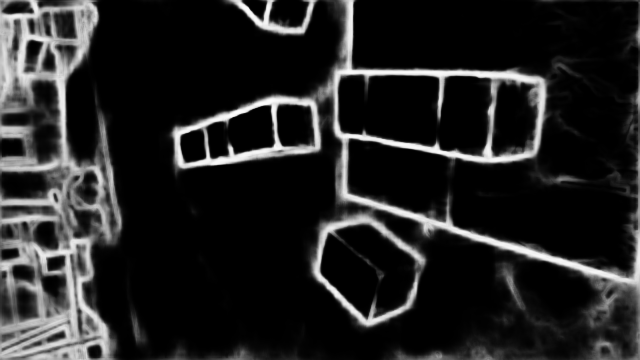
\includegraphics[width=\textwidth]{Holistically nested NN - 2.7s.png}
    \caption{Example of Holistically-Nested Edge Detection performance on the task image}
    \label{fig:hne}
\end{figure}

The algorithm was studied as an attempt to improve closed loop search reviewed in section 2.3. The problem of skeleton image resulted from Sobel filter is excessive number of loops generated by texture in order to store all the edges. As it deemed from the paper, the trained network generates edges that are part of detected objects only, hence algorithm output can be used directly for binary images to be traversed.

Example of the algorithm output is shown on Fig.\ref{fig:hne}. Average processing time for single image is 2.7 seconds on Intel Core i7-2630QM @ 2.00 GHz. The output image preserves strong edges and contains lower number of edges which are part of texture comparing to Sobel filter.

\subsection{You Only Look Once (YOLO)}

Neural network You Only Look Once, YOLO, is the-state-of-the-art neural network for real-time object detection. Since the first publish in 2015 in paper "You Only Look Once: Unified, Real-Time Object Detection" by Joseph Redmon et al., the proposed algorithm reached version number 4 in paper "YOLOv4: Optimal Speed and Accuracy of Object Detection" by Alexey Bochkovskiy et al. in 2020.

In this work pretrained on COCO dataset YOLO v2 tiny was taken for cuboid detection. All the cuboids were merged in a single class, hence, further color clarification may be needed. Dataset was made from more than 2000 images with augmentation in form of 4 different image size scales in range \{1, $\frac{2}{3}$, $\frac{1}{2}$, $\frac{1}{3}$\} and random image flipping with probability of 50\% is applied. Dataset was made in semi-automated way, proposed regions were guided by color range segmentation. Mean value per each channel for the whole dataset \{$\frac{88}{255}$, $\frac{113}{255}$, $\frac{113}{255}$\} is subtracted from individual images and divided by standard deviation for each channel \{$\frac{50}{255}$, $\frac{50}{255}$, $\frac{59}{255}$\}. Dataset of 9024 images in total is split on train and validation data in ratio 90:10 respectively. PyTorch was used to work with the network, the code is inherited from solution given in Autonomous Robotics class of Czech Technical University in Prague and modified in order to solve the task.

\begin{table}[htbp]
\centering
 \begin{tabular}{||c c c c c||} 
 \hline
 Layer & Channels (in x out) &  Kernel Size & Stride & Padding \\ [0.5ex] 
 \hline\hline
 Convolutional & 3x16 & 3x3 & 1 & 1 \\ 
 \hline
 MaxPool & & 2x2 & 2 & 2 \\
 \hline
 Convolutional & 16x32 & 3x3 & 1 & 1 \\ 
 \hline
 MaxPool & & 2x2 & 2 & 2 \\
 \hline
 Convolutional & 32x64 & 3x3 & 1 & 1 \\ 
 \hline
 MaxPool & & 2x2 & 2 & 2 \\
 \hline
 Convolutional & 64x128 & 3x3 & 1 & 1 \\ 
 \hline
 MaxPool & & 3x3 & 1 & 1\\
 \hline
 Convolutional & 128x256 & 3x3 & 1 & 1 \\ 
 \hline
 MaxPool & & 3x3 & 1 & 1\\
 \hline
 Convolutional & 256x512 & 3x3 & 1 & 1 \\ 
 \hline
 MaxPool & & 3x3 & 1 & 1\\
 \hline
 Convolutional & 512x1024 & 3x3 & 1 & 1 \\ 
 \hline
 Convolutional & 1024x1 & 1x1 & 1 & 1\\ [1ex] 
 \hline
\end{tabular}
\caption{YOLO neural network architecture}
\label{table:1}
\end{table}

The neural network architecture is present in Table \ref{table:1}. Batch normalization and Leaky ReLU with negative slope equal to 0.1, which follow every convolutional layer, excluding the final, were not shown for brevity. 

\begin{figure}[htbp]
    \centering
    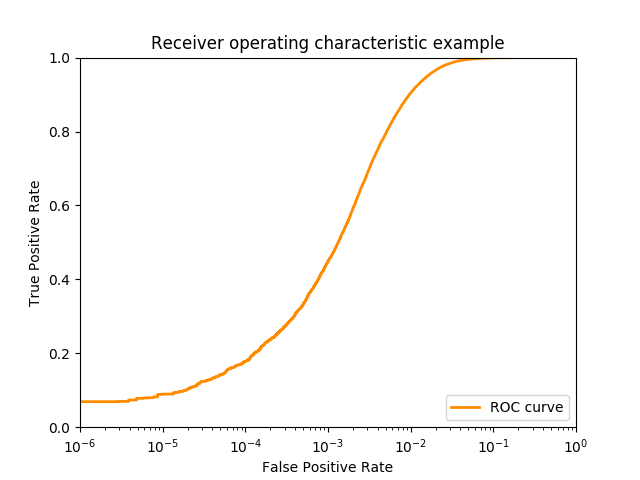
\includegraphics[width=\textwidth]{net_epoch100.png}
    \caption{Receiver operating characteristic for trained YOLO network}
    \label{fig:yolo-roc}
\end{figure}

Training has been done in batches of 2 images with learning rate $10^{-4}$ in 100 epochs. Stochastic Gradient Descent optimizer was taken, momentum was set to 0.9, weight decay $10^{-3}$. Receiver operating characteristic for the trained network is shown on Fig.\ref{fig:yolo-roc}. The network output for input image of size 3x360x640 pixels (Number of channels x Height x Width) is image of size 1x45x80, where every pixel value represent confidence of block detection in particular image region. In order to obtain cuboids area, output image is converted to binary in a way that all pixels with value less that confidence threshold are set to zero or to one otherwise. Then image is reshaped into original size and regions extracted.

The trained network was assessed on dataset it has never seen before, example of typical output is shown on Fig.\ref{fig:yolo}. In the most cases algorithm can detect blue and green object, some areas of red objects are detected in the most of cases (Fig.\ref{fig:y1}), however in some cases dark areas of any cuboid could be missed (Fig.\ref{fig:y3}). Objects such as computers or buildings, which has never used in training dataset, could yield a false positive (Fig.\ref{fig:y4} and \ref{fig:y6}), however, in most of cases it can correctly distinguish background (Fig.\ref{fig:y5}). It's supposed, that fine tuning of training parameters and dataset with higher number of images could help to achieve better training results. 

Average computation speed is 0.745 second on Intel Core i7-2630QM @ 2.00 GHz. It's known, that running the network on Graphic Processing Unit (GPU) or neural network accelerators such as Intel NCS2 and Coral USB accelerator could significantly improve the network computational speed results.

\begin{figure}[htbp]
     \centering
     \begin{subfigure}{0.475\textwidth}
         \centering
         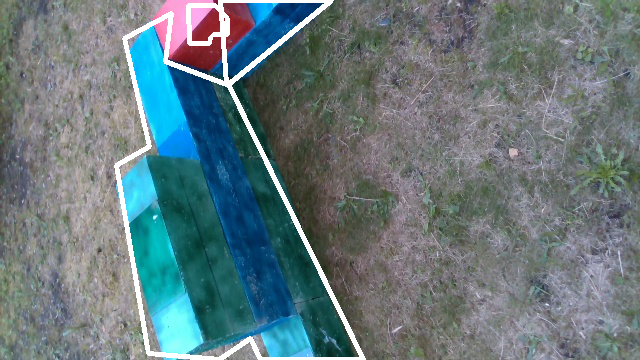
\includegraphics[width=\textwidth]{NN_0.png}
         \caption{Example of object detection}
         \label{fig:y1}
     \end{subfigure}
     \hfill
     \begin{subfigure}{0.475\textwidth}
         \centering
         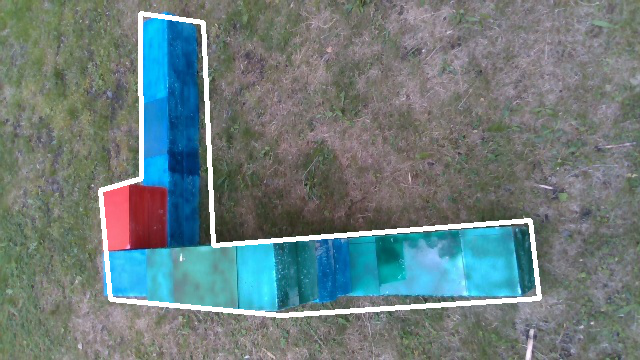
\includegraphics[width=\textwidth]{NN_1.png}
         \caption{Example of object detection}
         \label{fig:y2}
     \end{subfigure}
          \hfill
     \begin{subfigure}{0.475\textwidth}
         \centering
         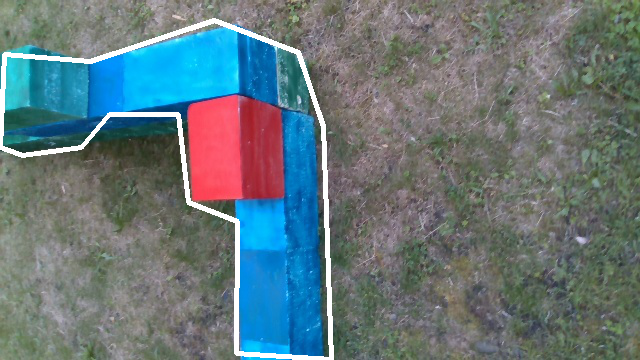
\includegraphics[width=\textwidth]{NN_2.png}
         \caption{Example of object detection}
         \label{fig:y3}
     \end{subfigure}
          \hfill
     \begin{subfigure}{0.475\textwidth}
         \centering
         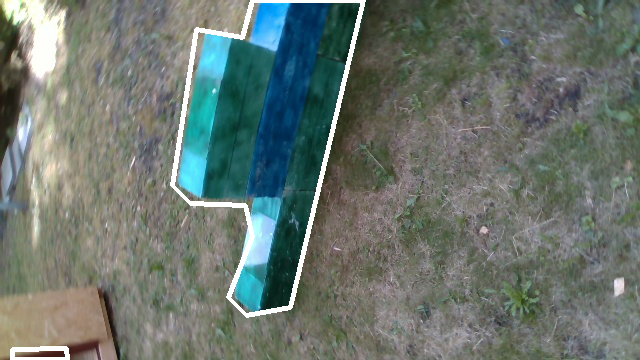
\includegraphics[width=\textwidth]{NN_3.png}
         \caption{Example of object detection}
         \label{fig:y4}
     \end{subfigure}
          \hfill
     \begin{subfigure}{0.475\textwidth}
         \centering
         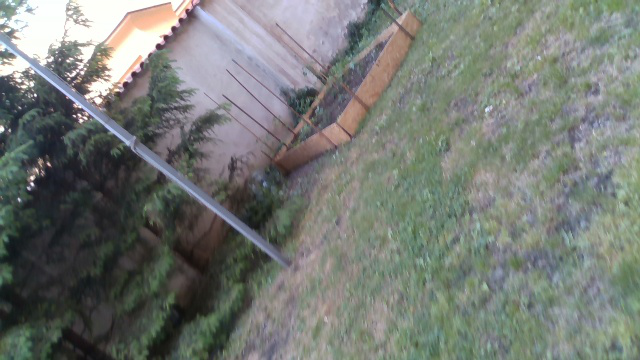
\includegraphics[width=\textwidth]{NN_6.png}
         \caption{Example of object detection}
         \label{fig:y5}
     \end{subfigure}
               \hfill
     \begin{subfigure}{0.475\textwidth}
         \centering
         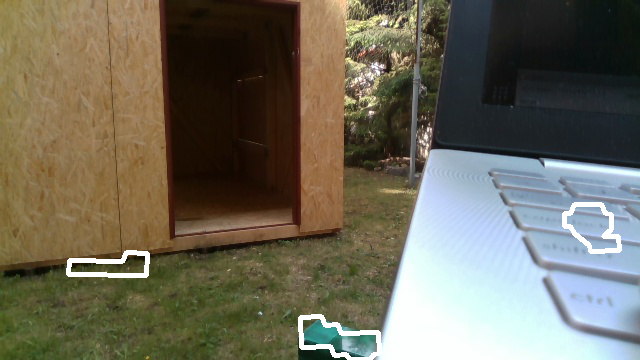
\includegraphics[width=\textwidth]{NN_5.png}
         \caption{Example of object detection}
         \label{fig:y6}
     \end{subfigure}
        \caption{Example of trained YOLO prediction (area inside white curves)}
        \label{fig:yolo}
\end{figure}

\section{Comparison of Color Image based Methods}
Four methods of color cuboid object detection were reviewed in this chapter. Since the algorithm shall be real-time, only those approaches, that have computational speed better than 1 Frame Per Second (FPS) could be used for the final solution. Computation time (in orders of second) for methods based on Color Segmentation (CS), GrabCut (GC), Search for a Closed Loop (CL), Holistically-Nested Edge detection (HNED) and YOLO v2 tiny neural network are shown in Table \ref{table:2}.

\begin{table}[h!]
\centering
 \begin{tabular}{||c c c c c c||} 
 \hline
 & CS & GC & CL & HNED & YOLO \\ [0.5ex] 
 \hline\hline
 Comp. time, s & $10^{-3}$ & $10^0$ & $10^1$ & $10^0$ & $10^{-1}$ \\ 
 [1ex] 
 \hline
\end{tabular}
\caption{Approximate computation time for the color image based methods in orders of second}
\label{table:2}
\end{table}

Only two methods - detection based on color segmentation and YOLO neural network, have computational speed better than 1 FPS. Moreover, it's known that computation time of neural network could be improved by usage of GPU or Neural Network Accelerators. Hence, the two potential methods were taken for detection quality assessment. The results are present in Table \ref{table:3}.

\begin{table}[h!]
\centering
 \begin{tabular}{||c c c ||} 
 \hline
  & Color segmentation & YOLO v2 tiny \\ [0.5ex] 
 \hline\hline
  False Positive & 4 & 19  \\ 
 \hline
  False Negative & 7 & 13  \\ 
 \hline
  True Positive & 347 & 331  \\ 
 \hline
 Precision & 0.989 & 0.946  \\ 
 \hline
 Recall & 0.980 & 0.962 \\ 
  \hline
 Avg. comp. time & 0.00496 & 0.80635 \\ 
 [1ex] 
 \hline
\end{tabular}
\caption{Detectors performance}
\label{table:3}
\end{table}

The assessment has been performed on dataset it has never been tested on before. The dataset recorded with unique illumination and weather. 100 random frames was taken for each method, total number of false positives and false negatives were calculated manually. True Positive was assigned if detected area is greater than $\frac{2}{3}$ of the cuboid object total area, otherwise the object results False Negative. False Positive is assigned in case area with a size above detection threshold is found and the area doesn't contain the cuboid object. Taking into account the fact, that the neural network is not capable to distinguish objects by color and in order to make the comparison fair, color information was out of scope of the assessment and region voting feature was off. Precision and Recall has been calculated in accordance with equations below.

\[ Precision = \frac{True\ Positives}{True\ Positives + False\ Positives} \]
\\
\[ Recall = \frac{True\ Positives}{True\ Positives + False\ Negatives} \]
\\
\\
In accordance with the algorithm comparison, the method based on Color Segmentation requires two orders less of computation time and demonstrates slightly better detection performance. Neural Network is a powerful tool, however, in case of a plain color object detection it was outperformed by the color segmentation algorithm. The color segmentation algorithm is set in order to achieve maximum recall, so no correct region of interest is missed, however, occasional missing is still occur. The algorithm will be taken as basis method for the fused approach and overall precision to be improved further.

\chapter{Methods of Detection for Depth Image}
\section{Depth Cameras and Depth Imaging}
Accurate depth imaging is relatively new technology and usually requires special hardware and algorithms to generate and process the data. Despite to color image, where every pixel has \{u, v, color\}, depth image consists of pixels, which have \{u, v, depth\}. Depth information could be obtained by different techniques, the most popular are based on time of flight and stereo triangulation.

Time of flight principle, as it comes from the name, is based on waves propagation and calculation of time till reflected waves return to the sensor. Taking into account the wave propagation speed (e.g. speed of light) and time travelled, we can compute distance to object \emph{D} as half of product of wave propagation speed \emph{c} and time of flight \emph{t}.

\[ D = \frac{c \times t}{2} \]

The principle is mainly used in LIDAR and sonar based imaging. LIDAR, which name is portmanteau of light and radar, is a device that generally consists of motor and rotating platform, which has light source and light sensor. Light source is typically laser light with maximum power and wavelength in safe for human eye range. Typical LIDAR rotates platform, which has light source and sensor. Light source propagates narrow band of light waves and calculate distance based on time what takes for reflected light to be detected by light sensor. Since platform is rotating, the measurement is performed in circular way with some angle step.

\begin{figure}[htbp]
    \centering
    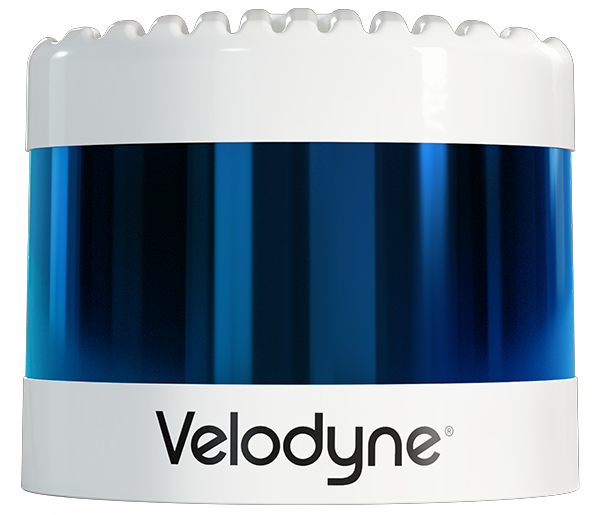
\includegraphics[width=0.75\textwidth]{Velodyne.png}
    \caption{Velodyne Alpha Prime LIDAR. Source \cite{velodyne}}
    \label{fig:lidar}
\end{figure}

However, it's worth to mention, that some versions of LIDAR today could have no moving parts and are used in a specific applications. Such LIDAR could be solid-state LIDAR, which is made in a form of phased array. Some versions of LIDAR have not just rotating platform for full angle view, but could rotate platofrom itself. Such improvement is beneficial in autonomous driving or mobile robotics, where objects around could be on various heights or agent's height is subject to change.

Another possible technique is stereo triangulation. The principle is based on stereo cameras with known mutual distance. Example of such camera is Intel RealSense D435 and it's shown on Fig.\ref{fig:d435}. Solving the correspondence problem, it's possible to get depth information for keypoints on epipolar line. However correspondence problem require vast amount of computational resources and some scenes could suffer from lack of correspondences, i.e. feature keypoints. Example of such scene could be a single color wall, ceiling or texture. With specific illumination, it's possible to obtain almost similar images on both cameras, hence correspondence problem couldn't be solved in such case without any additional scene information.

\begin{figure}[htbp]
    \centering
    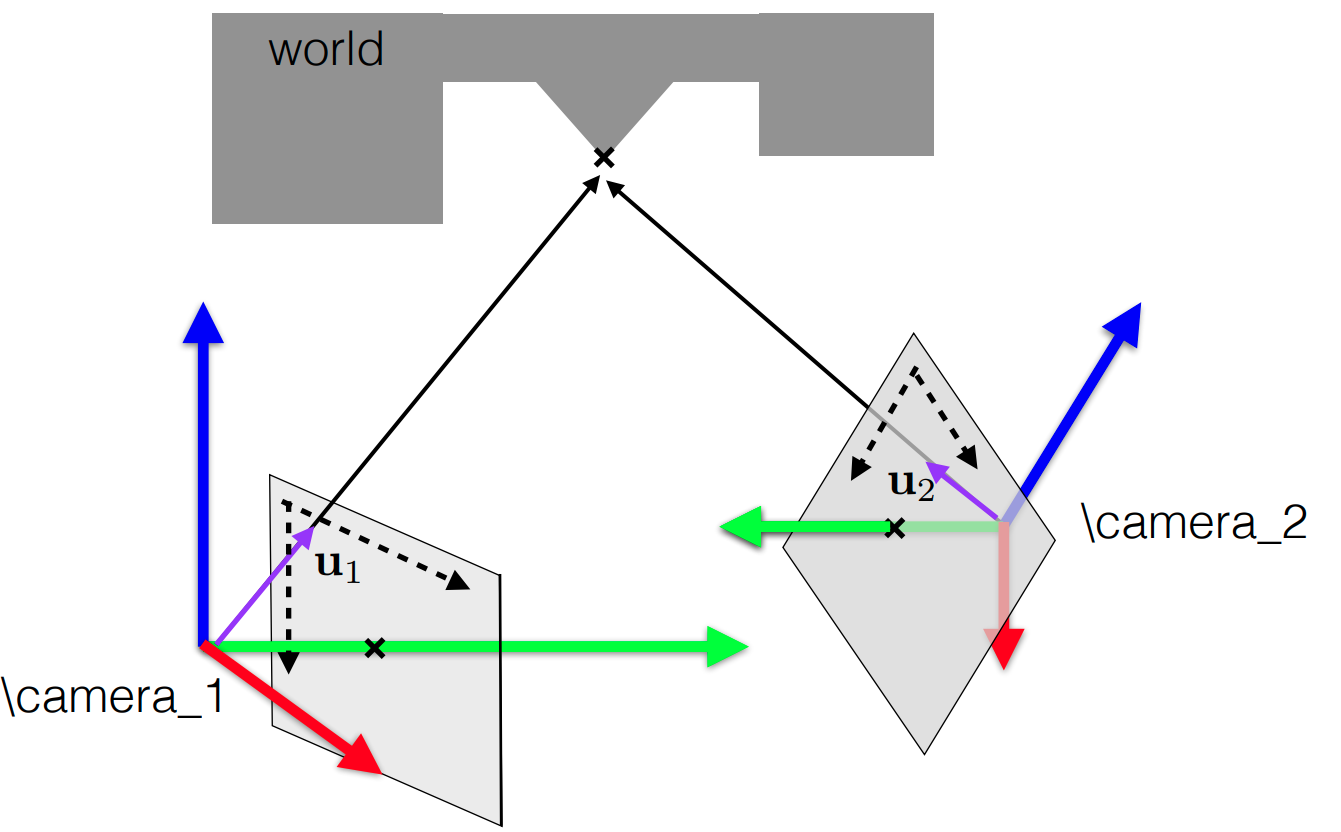
\includegraphics[width=0.85\textwidth]{stereo.png}
    \caption{Stereo triangulation. Source \cite{KZ-aro}}
    \label{fig:stereo}
\end{figure}

An additional information could be projected IR points with a specific pattern on scene. This could help to match keypoints in order to solve the correspondence problem. This technique is commonly used in RGB-D cameras such as Intel RealSense D435, Microsoft Kinect and others. The example of an image in IR range is shown on Fig.\ref{fig:ir_proj}.

\begin{figure}[htbp]
    \centering
    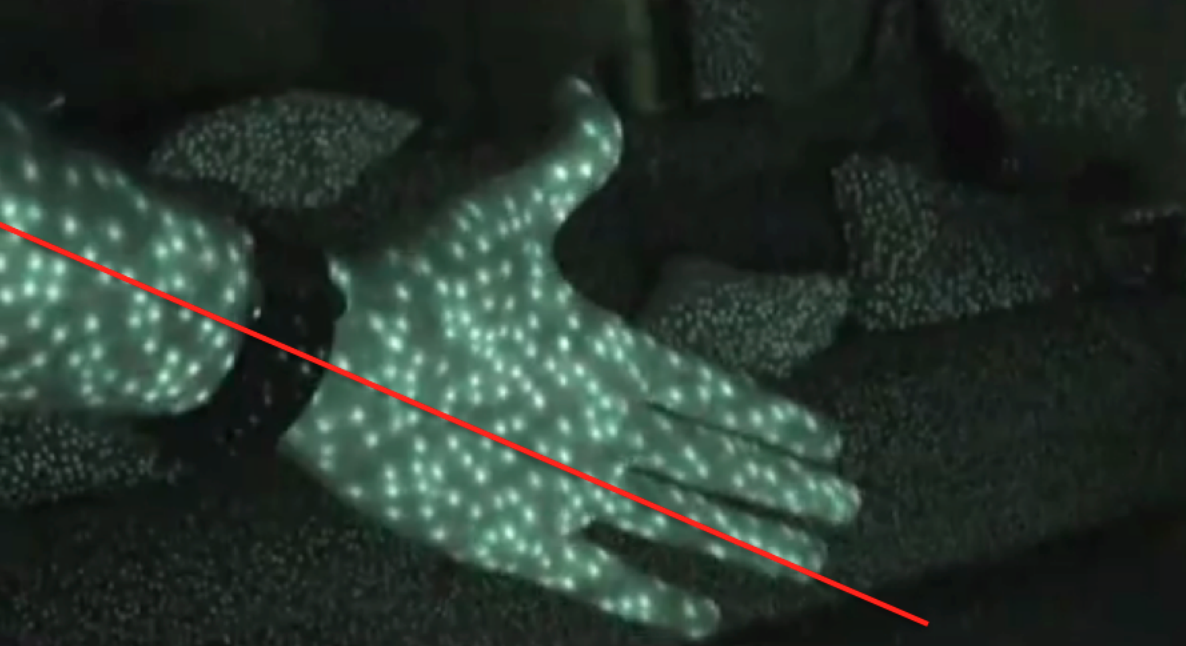
\includegraphics[width=\textwidth]{IR_projection.png}
    \caption{IR projection. Source \cite{KZ-aro}}
    \label{fig:ir_proj}
\end{figure}

Intel RealSense D435 camera was used as data source in this work. The camera creates a depth image as result of stereo triangulation. The scene is also projected by IR pattern to improve the stereo triangulation in low texture scene. Computation is performed by camera and output in form of images and camera calibration info is transmitted via USB. 

\begin{figure}[htbp]
    \centering
    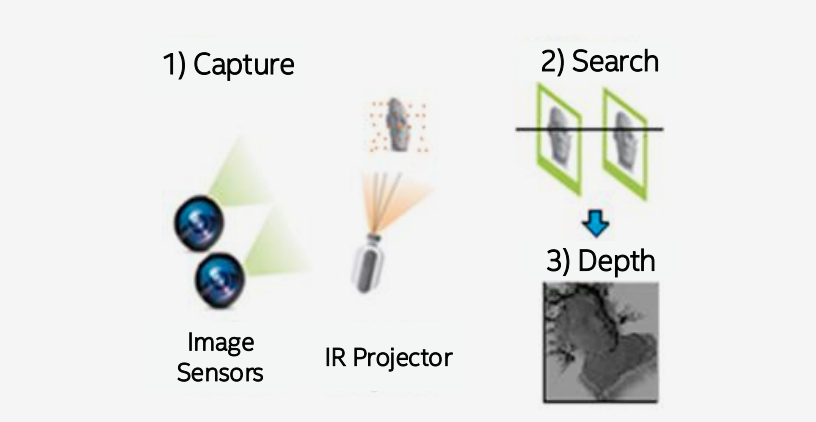
\includegraphics[width=\textwidth]{I_RS_1.png}
    \caption{Active Infrared (IR) Stereo Vision Technology. Source \cite{intel}}
    \label{fig:I_RS_1}
\end{figure}

The camera calculates depth for every pixel as distance from the center of left and right image sensors to the object. Depth pixel values are used to compose the depth frame.

\begin{figure}[htbp]
    \centering
    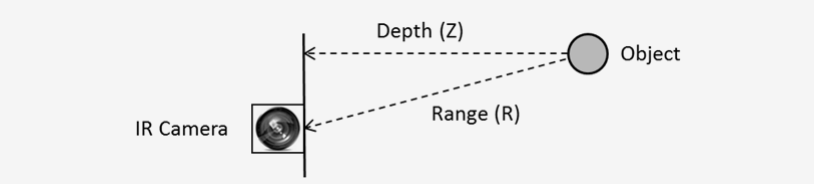
\includegraphics[width=\textwidth]{I_RS_2.png}
    \caption{Depth Measurement (Z) versus Range (R). Source \cite{intel}}
    \label{fig:I_RS_2}
\end{figure}

\section{Conversion of Depth Image into a Point Cloud}

In order to use the Point Cloud Library, the depth image should be converted into a point cloud. The conversion requires Projection matrix P to be known. 

\[P = \begin{bmatrix}
fx & 0 & cx & Tx\\
0 & fy & cy & Ty\\
0 & 0 & 1 & 0
\end{bmatrix}, \]

where fx, fy are focal lengths, cx, cy are principal point and Tx, Ty are position of the optical center of the second camera in the first camera's frame \cite{ros}.

Every pixel with coordinates \{u, v\} of depth image with distance \emph{d} as its pixel value could be converted to a point with coordinates \{x, y, z\} using pinhole camera model with following equation

\[\begin{bmatrix}
x\\
y\\
z
\end{bmatrix} = \begin{bmatrix}
(d \cdot (u - cx) - Tx) \cdot fx^{-1}\\
(d \cdot (u - cy) - Ty) \cdot fy^{-1}\\
d
\end{bmatrix} \]

The conversion is performed in ROS environment. Developed by Willow Garage package depth\_image\_proc provides a nodelet for depth image to point cloud conversion. The depth image to point cloud conversion example is shown of Fig.\ref{fig:pc-conv}.

\begin{figure}[htbp]
     \centering
     \begin{subfigure}{0.475\textwidth}
         \centering
         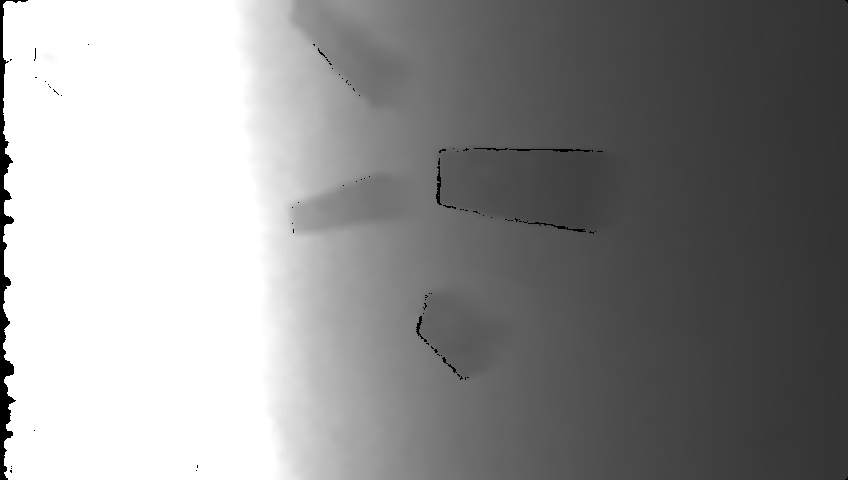
\includegraphics[width=\textwidth]{depth_example.jpg}
         \caption{Depth image}
         \label{fig:de}
     \end{subfigure}
     \hfill
     \begin{subfigure}{0.475\textwidth}
         \centering
         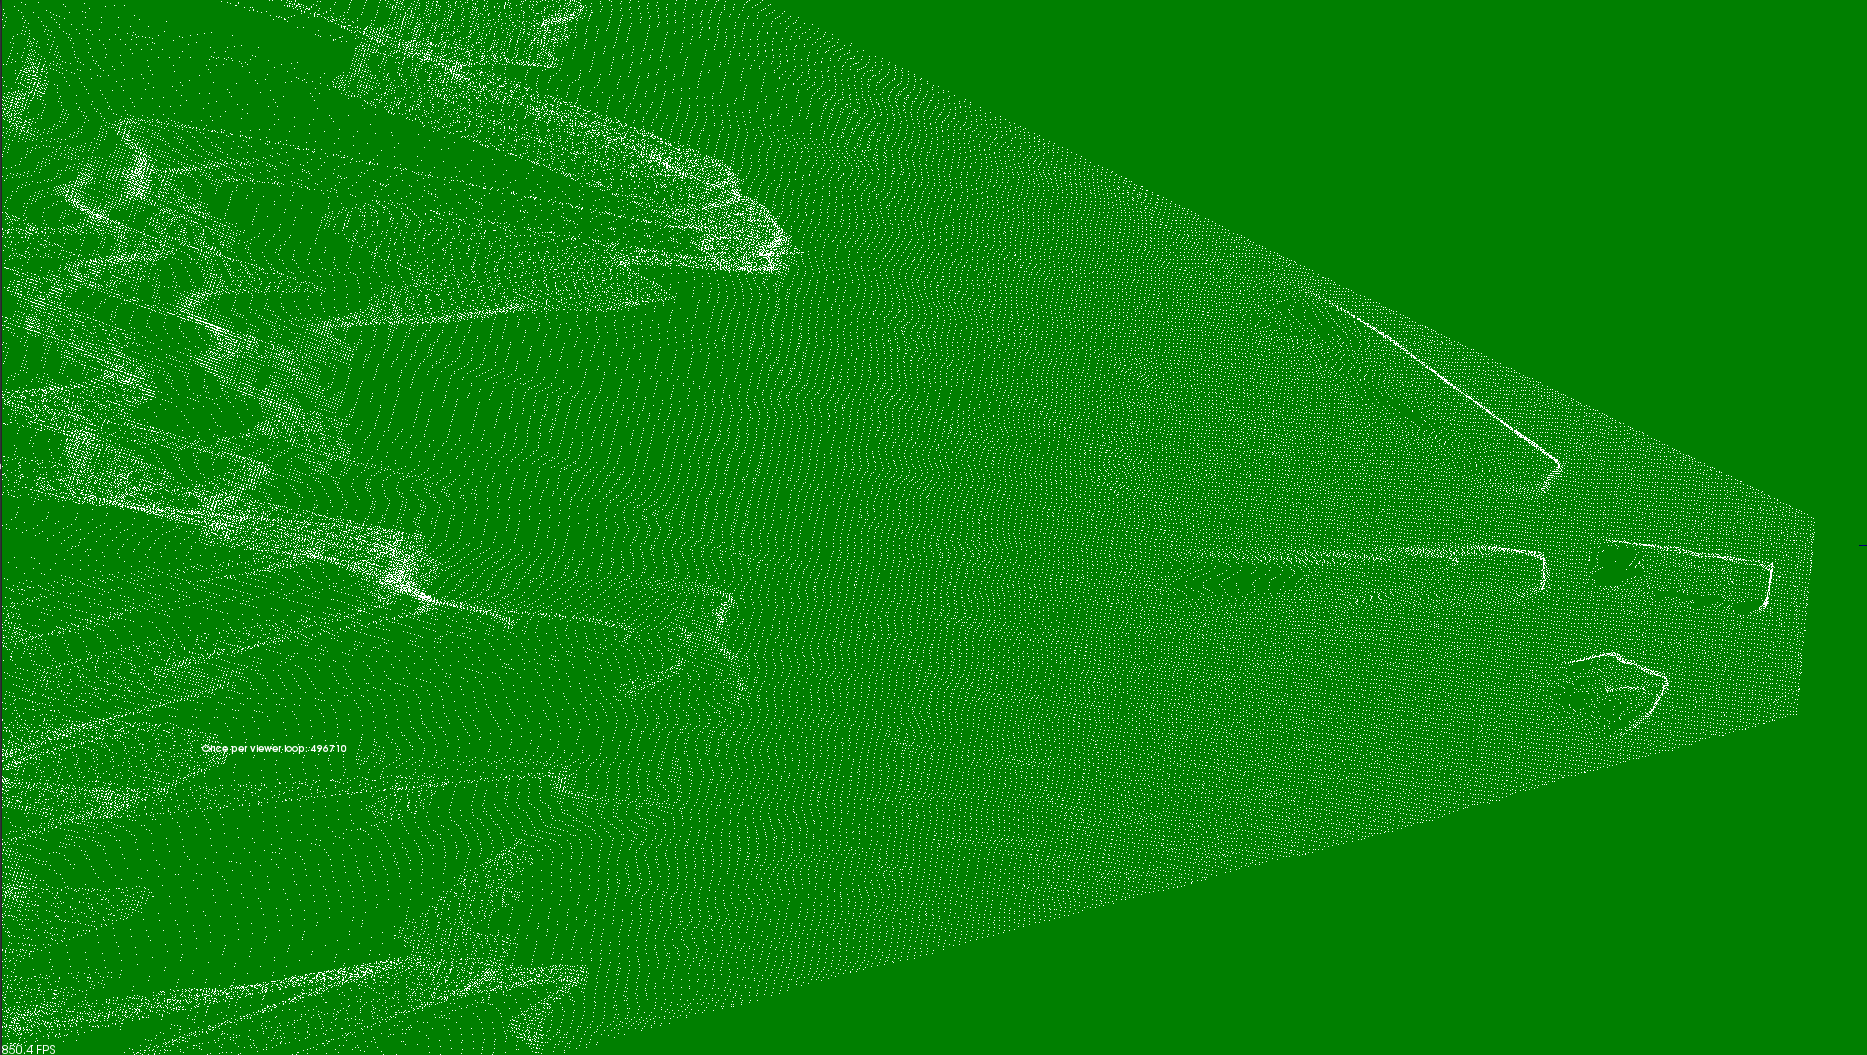
\includegraphics[width=\textwidth]{point_cloud_2.png}
         \caption{Converted point cloud}
         \label{fig:pce}
     \end{subfigure}

        \caption{Example of depth image to point cloud conversion}
        \label{fig:pc-conv}
\end{figure}

\section{Algorithm based on Point Cloud} \label{pca}

Once point cloud is obtained, it could be segmented on planes using RANSAC algorithm. The plane with highest number of points is considered as a ground plane. Every other plane is checked as a cuboid candidate. To process the candidate, every segmented plane cloud should be clustered to separate cuboid objects and possible noise or errors. Every cluster should be also checked in terms of area size and plane height related to ground. The complete algorithm is provided in algorithm \ref{depth-alg} section.

\begin{algorithm}
\caption{Algorithm based on Point Cloud}\label{depth-alg}
\begin{algorithmic}[1]
\State $ground \gets \emptyset$
\State $result \gets \emptyset$
\State $points \gets all\_points$
\State $planes \gets RANSAC(points,\ dist\_thresh,\ min\_points)$
\State $planes \gets sort\_by\_size(planes)$
\For{$every\ plane\ in\ planes$}
\State $if (ground = \emptyset):\ ground \gets plane$
\State $if (plane\ != ground):\ clusters \gets get\_clusters(plane)$
\For{$every\ cluster\ in\ clusters$}
\State $dist \gets get\_dist(cluster, ground)$
\State $if\ (dist < min\_dist)\ or\ (dist > max\_dist): continue$
\State $area \gets get\_area(cluster)$
\State $if (area < min\_area)\ or\ (area > max\_area): continue$
\State $results \gets cluster,\ get\_center(cluster)$
\EndFor
\EndFor
\end{algorithmic}
\end{algorithm}

Average processing time for a single point cloud is 0.20 second on Intel Core i7-2630QM @ 2.00 GHz. 

\subsection{Plane Segmentation using RANSAC}

Since the scene is supposed to be composed of flat ground and man-made objects, which are also deemed to be flat shape (cuboids, wall), it's possible to segment the scene on planes and perform further processing on found planes. However, the scene could contain terrains and algorithm shall correctly distinguish them.

Plane segmentation method used in this work is based on RANSAC, Random Sample Consensus, approach. Algorithm is non-determenistic approach to obtain parametric model based on random points selected. It was published by Fischler and Bolles in 1981. The algorithm picks random points and computes plane equation by solving system of linear equations. The plane equation in form of $Ax + By + Cz + D = 0$ is applied to the rest points and number of inliers is computed. Inlinier is a point which lays on computed plane or within given threshold from the plane. The process repeats given number of iteration times and plane equation with maximum number of inliers is stored. Algorithm could be halted before the maximum number of iterations has been reached in case it's already equal or greater than 

\[ iter \geq \frac{\ln{(1 - p)}}{\ln{(1 - w^n)}}, \]

where p stands for confidence in range [0,1] (typically 0.95), w - ratio of inliers to total number of points, n - random sample size.

RANSAC algorithm could be illustrated on 2D example for simplification purpose. As it shown on Fig.\ref{fig:ransac}, the set of points should be processed in order to obtain 2D line. The data not only consists of points, which truly make the line, but also noise, errors or irrelevant data points. The algorithm randomly picks points and compute line equation. The line equation could be obtained, for example, by the Least Squares method. Then algorithm applies the equation and given threshold, margins, and computes number of points which lay inside the margins. Those points are named \emph{inliers}. Algorithm repeats until parametric model with the highest number of inliers is found.

\begin{figure}[htbp]
     \centering
     \begin{subfigure}{0.475\textwidth}
         \centering
         \includegraphics[width=\textwidth]{RANSAC_bad.png}
         \caption{Model with low number of inliers}
         \label{fig:ransac-a}
     \end{subfigure}
     \hfill
     \begin{subfigure}{0.475\textwidth}
         \centering
         \includegraphics[width=\textwidth]{RANSAC_good.png}
         \caption{Model with high number of inlliers}
         \label{fig:ransac-b}
     \end{subfigure}

        \caption{Example of RANSAC algorithm for linear model in 2D. Source \cite{MPV}}
        \label{fig:ransac}
\end{figure}


\begin{algorithm}
\caption{RANSAC algorithm}\label{ransac}
\begin{algorithmic}[1]
\State $points \gets all\_points$
\State $best\_model \gets \emptyset$
\State $max\_inl \gets 0$
\For{iter in $max\_num\_of\_iter$ }

\State $rand\_points \gets random\_points(points, num\_of\_points)$
\State $model \gets compute\_model(rand\_points)$
\State $inl \gets compute\_inl(model, points)$
\State $if\ inl > max\_inl: best\_model \gets model, max\_inl \gets inl$
\State $if\ iter \geq \frac{\ln{(1 - p)}}{\ln{(1 - (inl/points)^(num\_of\_points))}}: \ break$
\EndFor

\end{algorithmic}
\end{algorithm}


The algorithm is used to segment planes on given point cloud is provided in PCL library. Example of plane segmentation result is shown on Fig.\ref{fig:plane_segm}. For further processing it's supposed, that plane with the highest number of point is the ground plane. Parametric model in form of $Ax + By + Cz + D = 0$ is stored for further computations.

\begin{figure}[htbp]
    \centering
    \includegraphics[width=\textwidth]{segmented_scene.png}
    \caption{Plane segmentation example (planes have individual color)}
    \label{fig:plane_segm}
\end{figure}

\subsection{Point Clustering}

Since scene could have several objects, which compose a single plane, e.g. tops of several cuboid objects or cuboid object with random textures on the same height aside, algorithm shall correctly distinguish those object and segment obtained plane on clusters to process them individually. The algorithm used is based on Euclidean distances and forms clusters of points which lays on some short distance \emph{$d_{th}$} to each other.

\begin{algorithm}
\caption{Euclidean clustering. Source \cite{euc}}\label{euc}
\begin{algorithmic}[1]
\State $P \gets k-d\ representation\ of\ point\ cloud$
\State $C \gets \emptyset,\ Q \gets \emptyset$

\For{every point $p_i \in P$ }
\State $Q \gets p_i$
\For{every point  $p_i \in Q$ }
\State $P_i^k \gets neighbors\ of\ p_i\ in\ a\ sphere\ with\ radius\ r < d_{th}$
\For{every point  $p_i^k \in P_i^k$ }
\State $if p_i^k\ is\ not\ checked: Q \gets p_i^k$
\EndFor
\EndFor
\State $C \gets Q,\ Q \gets \emptyset$
\State $if\ no\ new\ points:\ break$
\EndFor

\end{algorithmic}
\end{algorithm}


The algorithm used is the part of PCL and it was proposed by Radu Bogdan Rus in 2009 in his dissertation "Semantic 3D Object Maps for Everyday Manipulation in Human Living Environments", Technical University of Munich. Main features of the algorithm that it takes K-d representation of the point cloud dataset P and split split unorganized point cloud model into smaller parts to improve overall computation speed.


\begin{figure}[htbp]
    \centering
    \includegraphics[width=\textwidth]{euc_cluster.png}
    \caption{Example of point clustering (clusters have individual color)}
    \label{fig:euc}
\end{figure}

\subsection{Plane Equation Calculation}

Plane equation in form of $Ax + By + Cz + D = 0$ could be obtained from at least three points. Those points shall not lay on a line. System of linear equations is obtained from such points, approximated solution of the system will be the plane equation.

\begin{figure}[htbp]
    \centering
    \includegraphics[width=\textwidth]{plane_eq.png}
    \caption{Plane made of three points}
    \label{fig:plane_eq}
\end{figure}

\[
\begin{cases} A \cdot x_1 + B \cdot y_1 + C \cdot z_1  + D = 0 \\ A \cdot x_2 + B \cdot y_2 + C \cdot z_2  + D = 0 \\ A \cdot x_3 + B \cdot y_3 + C \cdot z_3  + D = 0 \end{cases}
\]

What can be also solved in the matrix form

\[\begin{bmatrix}
x_1 & y_1 & z_1 & 1\\
x_2 & y_2 & z_2 & 1\\
x_3 & y_3 & z_3 & 1\\
\end{bmatrix} \cdot \begin{bmatrix}
A\\
B\\
C\\
D
\end{bmatrix} = \begin{bmatrix}
0\\
0\\
0
\end{bmatrix}\]

Plane equation is used in RANSAC algorithm for plane segmentation. Proposed approach is one of the possible solutions for the given problem. Exact method depends on implementation.

\subsection{Distance to Plane Calculation}
Once individual point cluster is obtained, it's possible to check it's properties to define if the cluster is cuboid object. From geometric point of view, the cuboid object is composed from several flat planes, top plane has specific area and specific height, i.e. distance to ground.

\begin{figure}[htbp]
    \centering
    \includegraphics[width=\textwidth]{point-plane-dist.png}
    \caption{Point-plane distance d}
    \label{fig:plane_dist}
\end{figure}


Distance \emph{d} of point \emph{p} with parameters \{$p_x, p_y, p_z$\} to plane defined as $Ax + By + Cz + D = 0$ could be calculated as

\[ d = \frac{\mid A \cdot p_x + B \cdot p_y + C \cdot p_z + D \mid}{\sqrt{A^2 + B^2 + C^2}} \]

Since plane is obtained using RANSAC algorithm with some threshold $d_{th}$, plane points could have legit height in following range 

\[ [h_{cuboid} - d_{th} \pm s_{noise}, h_{cuboid} \pm s_{noise}], \]

where $h_{cuboid}$ is cuboid height, $s_{noise}$ is depth camera sensor noise.

It's necessary to assess a set of points of size \emph{n} of examined cluster to define if it could be cuboid top plane. For such purpose it's necessary to calculate minimum, maximum and median values. Minimal value couldn't be less than $(h_{cuboid} - d_{th} \pm s_{noise})$ and maximum value greater than $(h_{cuboid} \pm s_{noise})$. Meanwhile median value should be greater than arithmetical average of minimum and maximum values. If the plane's height is out of range, then plane is rejected. Such approach helps to reject planes, which doesn't belong to the cuboid object - planes that are not parallel to ground or have non-flat surfaces.


\subsection{Polygon Area Calculation}

In order to obtain detected plane area, point cloud, that represents the plane, should be converted to a polygon. Polygon is a plane figure which represents outer contour of the point cloud. Polygon consists of n points, where each point \emph{$p_i$} has \{$x_i$, $y_i$, $z_i$\} coordinates. Plane area \emph{A} could be obtained as following

\begin{figure}[htbp]
    \centering
    \includegraphics[width=\textwidth]{poly-area.png}
    \caption{Polygon area A}
    \label{fig:poly_area}
\end{figure}

\[ A = \frac{1}{2} \cdot ( \begin{bmatrix}
x_1\\
y_1\\
z_1
\end{bmatrix} \cdot \begin{bmatrix}
x_2\\
y_2\\
z_2
\end{bmatrix} + \begin{bmatrix}
x_2\\
y_2\\
z_2
\end{bmatrix} \cdot \begin{bmatrix}
x_3\\
y_3\\
z_3
\end{bmatrix} + ... + \begin{bmatrix}
x_n\\
y_n\\
z_n
\end{bmatrix} \cdot \begin{bmatrix}
x_1\\
y_1\\
z_1
\end{bmatrix} )  \]

Polygon area is important property, which helps to define whether the given point cloud represents the block or not. Objects of different colors are assumed to have different surface area. The area also serves to define whether the area could represent the object partially and, hence, become a potential region.

\subsection{Polygon Center Calculation}
Detected object center could be an algorithm output as an target point for magnet holder. Calculation of detected plane center requires a polygon of the plane point cloud. The center point \{$x_c$, $y_c$, $z_c$\} is calculated as arithmetical mean of the polygon points coordinates.

\begin{figure}[htbp]
    \centering
    \includegraphics[width=\textwidth]{poly_center.png}
    \caption{Polygon center $C_{xyz}$}
    \label{fig:poly_ctr}
\end{figure}

\[\begin{bmatrix}
x_c\\
y_c\\
z_c
\end{bmatrix} = \begin{bmatrix}
n^{-1} \cdot \sum_{i=1}^{n} x_i\\
n^{-1} \cdot \sum_{i=1}^{n} y_i\\
n^{-1} \cdot \sum_{i=1}^{n} z_i
\end{bmatrix} \]



\section{Summary}
Proposed algorithm could robustly detect cuboid objects on a given scene. With the assumed cuboid objects geometrical properties, the algorithm gives no false positive results, however, due to sensor noise and stereo triangulation imperfection, objects on a high distance, more than 3 meters, do suffer from geometrical distortions and hence, are rejected by the algorithm. To avoid high number of false negatives, a wider geometrical limits were introduced. It's known, that geometric properties are always getting less than they are, hence appropriate compensation could be introduced further. Moreover, algorithm can distinguish multiple objects on scene and return detection result as found cuboid object top plane centers.

\chapter{Color and Depth Methods Fusion}
\section{Sensor Fusion Algorithm}

As it was mentioned in previous chapters, color segmentation approach with wide color ranges could yield good recall and precision with low computation time. However, wide color ranges could also result false positives, which should be filtered out. Geometrical verification in form of algorithm that is based on point cloud could be used to reject false positives. Such sensor fusion is deemed to improve overall algorithm precision. 

The algorithm starts with color segmentation. Detected regions are checked on overlapping and region voting is performed. Boundary box for every cuboid object candidate is calculated and enlarged in order to include object background information. Boundary box coordinates are converted from RGB camera coordinates to depth camera coordinates using Intrinsic camera matrices K for both RGB and depth cameras.


\[K = \begin{bmatrix}
fx & 0 & cx\\
0 & fy & cy\\
0 & 0 & 1
\end{bmatrix}, \]

where fx, fy are focal lengths and cx, cy are principal point. The Intrinsic matrix is unique for every image sensor and calculated during camera calibration. Projection of a 3D point on image plane equation could be used for RGB and Depth cameras mapping.

\[ \lambda \begin{bmatrix}
u\\
v\\
1
\end{bmatrix} = K \cdot \begin{bmatrix}
p_x\\
p_y\\
p_z
\end{bmatrix} \]

\[ K^{-1} \cdot \lambda \begin{bmatrix}
u\\
v\\
1
\end{bmatrix} = \begin{bmatrix}
p_x\\
p_y\\
p_z
\end{bmatrix}\]

\[ \lambda \begin{bmatrix}
u_D\\
v_D\\
1
\end{bmatrix} = K_D \cdot K_C^{-1} \cdot \lambda \begin{bmatrix}
u_C\\
v_C\\
1
\end{bmatrix} \]

\[ \begin{bmatrix}
u_D\\
v_D\\
1
\end{bmatrix} = K_D \cdot K_C^{-1} \cdot \begin{bmatrix}
u_C\\
v_C\\
1
\end{bmatrix} \]



Every cuboid object candidate region is cropped from depth image and converted to a point cloud. Algorithm based on point cloud is used to confirm or reject the region and obtain object top plane centres. 

\begin{algorithm}
\caption{Color and Depth Methods Fusion}\label{sens-f}
\begin{algorithmic}[1]

\State $image\_c \gets input\ color\ image$
\State $image\_d \gets input\ depth\ image$
\State $color\_range[r,g,b] \gets HSV\ color\ ranges$
\State $color\_regions \gets \emptyset$
\State $result \gets \emptyset$

\State $hsv\_image \gets cv2.cvtColor(image\_c, cv2.COLOR\_RGB2HSV)$
\For{each color in $color\_range$ }
\State $candidates \gets cv2.inRange(hsv\_image, color\_range[color])$
\For{each candidate in $candidates$ }
\State $if\ getArea(candidate) < area\_threshold:\ continue$
\State $polyline \gets getPolyline(candidate)$
\State $if\ len(polyline) > lines\_threshold:\ continue$
\State $color\_regions \gets candidate$
\EndFor
\EndFor


\State $candidates \gets sort(color\_regions)$
\For{each candidate in $candidates$ }
\State $iff\ candidate \cup dummy\_image > area\_threshold:\ continue$
\State $dummy\_image[candidate] \gets 1$
\State $x_1, y_1, x_2, y_2 \gets enlarged\_bbox(candidate)$
\State $depth\_crop \gets image\_d[x_1 - x_2 : y_1 - y_2]$
\State $avg\_depth = average(depth\_crop)$
\State $if\ (avg\_depth < min\_depth): continue$
\State $points \gets get\_point\_cloud(depth\_crop)$
\State $ground \gets \emptyset$


\State $planes \gets RANSAC(points,\ dist\_thresh,\ min\_points)$
\State $planes \gets sort\_by\_size(planes)$
\For{$every\ plane\ in\ planes$}
\State $if (ground = \emptyset):\ ground \gets plane$
\State $if (plane\ != ground):\ clusters \gets get\_clusters(plane)$
\For{$every\ cluster\ in\ clusters$}
\State $dist \gets get\_dist(cluster, ground)$
\State $if\ (dist < min\_dist)\ or\ (dist > max\_dist): continue$
\State $area \gets get\_area(cluster)$
\State $if (area < min\_area)\ or\ (area > max\_area): continue$
\State $result \gets get\_center(cluster)$
\EndFor
\EndFor
\EndFor

\end{algorithmic}
\end{algorithm}

The fused algorithm is composed from Color Segmentation, Region Voting and Point Cloud Algorithms \ref{hsv}, \ref{reg-vote} and \ref{depth-alg} respectively. Detailed description of algorithm steps are present in Sections \ref{csa} and \ref{pca}.

The solution is designed to work in ROS environment and based on synchronised color and depth frames. Algorithm segment images on color and perform region voting to reject overlapped candidates. Then it assess distance to object. In case object is too close and hence, observed only partly, the candidate is rejected in order to process only objects, which are complete in the field of view. Algorithm output are centers of detected candidates, therefore, it gives relative location for object handling algorithm by passing coordinates of cuboid object metal plate for holding. Example of fused algorithm detection is shown on Fig.\ref{fus-alg-ex}

\begin{figure}[htbp]
    \centering
    \includegraphics[width=\textwidth]{fused_alg_ex.png}
    \caption{Example of cuboid object detection with fused algorithm}
    \label{fus-alg-ex}
\end{figure}

Detected object centers, which could be the target point for cuboid object handling algorithm, are shown as circles with appropriate color. The detected centers are main output of the algorithm, because it can direct the UAV. Colored boundary box are potential regions, i.e. regions, which resulted by Color Segmentation algorithm, but during geometrical verification a plane within distance threshold was found, however, its area is below minimal surface area threshold. It's likely, that such region is a partly observable object. The regions could be valuable in case no object center were detected and it can direct the UAV to explore the region.

\section{Algorithm performance}

Algorithm performance was assess on obtained dataset of total size more than 2900 frame pairs of color and depth images. During the assessment following parameters were assessed:
\begin{itemize}
  \item Number of correctly projected centers, which are truly on metal plate for handling
  \item Number of drifted projected centers, which are located on the object, but not on metal plate for handling
  \item Number of incorrect projected centers, which are located not on the object
  \item Number of projected centers, which have incorrect color
  \item Total number of objects, which are completely observed in frame
  \item Number of potential regions, which are passed by color segmentation filter, but found object area is less that minimal threshold (partly observed objects)
  \item Average processing time for all frames
  \item Average processing time for frames, which require geometrical verification and yield center projection
\end{itemize}

\begin{table}[h!]
\centering
 \begin{tabular}{||c | c | c ||} 
 \hline
  & \vtop{\hbox{\strut Number of detection,}\hbox{\strut      absolute}} & \vtop{\hbox{\strut Number of detection,}\hbox{\strut    relative to total}} \\ [0.5ex] \hline\hline
  Correctly projected center & 234 & 36.0\%  \\ 
 \hline
  Drifted projected center & 35 & 5.4\%  \\ 
 \hline
  Incorrect projected center & 0 & 0.0\%  \\ 
 \hline
 \vtop{\hbox{\strut Projected center of}\hbox{\strut incorrect color}}  & 0 & 0.0\%  \\ 
 \hline
 Total number of objects & 650 & 100.0\% \\ 
 \hline
 Potential regions & 1241 & 190.9\% \\ 
 \hline\hline
 \vtop{\hbox{\strut Avg. comp. time}\hbox{\strut for all frames, s}}  & \multicolumn{2}{|c||}{0.0343}\\ 
 \hline
 \vtop{\hbox{\strut Avg. comp. time for}\hbox{\strut geom. verified frames, s}}  & \multicolumn{2}{|c||}{0.1130} \\ 
 [1ex] 
 \hline
\end{tabular}
\caption{Final Detector Performance}
\label{table:final_perf}
\end{table}

Algorithm can give a correct location for block handling in 36\% of detections. Drifted location is given in 5.4\%, however it can be improved by averaging of the location, which is resulted from several frames. In given dataset the algorithm didn't return any incorrect locations. Moreover, all the color predictions was correct. Algorithm provides high number of potential regions - the number exceeds 100\% because total number of objects is based only on blocks, which are completely in the image frame, however potential region could be correctly detected with partially observed object.
Average computation time for the whole dataset is 0.0343 second on Intel Core i7-2630QM @ 2.00 GHz. Algorithm doesn't perform the geometrical verification in most of frames, because object are either too close, so they aren't in the frame completely, or too far from the UAV and, hence, suffer from geometrical distortion on depth image. Average computation time for frames, which resulted correct center projection is 0.1130 second, what gives 8.85 FPS on the mentioned machine.
Taking only correct center projections as true positive and total number of objects on scene as summation of true positive and false negative, yields algorithm recall equal to 36\%. Considering the output has no incorrect projected centers, the algorithm achieves 100\% algorithm's precision.

\begin{figure}[htbp]
     \centering
     \begin{subfigure}{0.475\textwidth}
         \centering
         \includegraphics[width=\textwidth]{Fin_0.png}
         \caption{Example of object detection}
         \label{fig:f1}
     \end{subfigure}
     \hfill
     \begin{subfigure}{0.475\textwidth}
         \centering
         \includegraphics[width=\textwidth]{Fin_1.png}
         \caption{Example of object detection}
         \label{fig:f2}
     \end{subfigure}
          \hfill
     \begin{subfigure}{0.475\textwidth}
         \centering
         \includegraphics[width=\textwidth]{Fin_3.png}
         \caption{Example of object detection}
         \label{fig:f3}
     \end{subfigure}
          \hfill
     \begin{subfigure}{0.475\textwidth}
         \centering
         \includegraphics[width=\textwidth]{Fin_5.png}
         \caption{Example of object detection}
         \label{fig:f4}
     \end{subfigure}
          \hfill
     \begin{subfigure}{0.475\textwidth}
         \centering
         \includegraphics[width=\textwidth]{Fin_6.png}
         \caption{Example of object detection}
         \label{fig:f5}
     \end{subfigure}
    \hfill
     \begin{subfigure}{0.475\textwidth}
         \centering
         \includegraphics[width=\textwidth]{fused_alg_ex.png}
         \caption{Example of object detection}
         \label{fig:f6}
     \end{subfigure}
    \hfill
     \begin{subfigure}{0.475\textwidth}
         \centering
         \includegraphics[width=\textwidth]{Fin_9.png}
         \caption{Example of object detection}
         \label{fig:f7}
     \end{subfigure}
                    \hfill
     \begin{subfigure}{0.475\textwidth}
         \centering
         \includegraphics[width=\textwidth]{Fin_10.png}
         \caption{Example of object detection}
         \label{fig:f8}
     \end{subfigure}
        \caption{Example of the final solution detection results}
        \label{fig:fus-alg}
\end{figure}

The results present of Fig.\ref{fig:fus-alg} represents typical correct detection results. In majority of cases cases geometrical verification results false negative even if the object is close enough and it's complete in the field of view - Fig.\ref{fig:f1}, \ref{fig:f5} and \ref{fig:f8}. The main reasons are imperfection of depth imaging process and algorithm optimization in order to maintain real-time computational speed. The algorithm parameters were set with consideration of high precision and it still gives acceptable recall.

Algorithm is able to distinguish several objects in the single color region - Fig.\ref{fig:f1} and \ref{fig:f6}. Algorithm can also detect correct object even in case of partly incorrect color due to objects superposition, initially wrong surface color or light reflection - Fig.\ref{fig:f6}. 

\section{Possible Improvements}
The main disadvantages of the proposed solution are not high enough recall and computational speed. The recall could be improved by more sophisticated depth imaging. One of such approaches could be multi planar LIDAR - the LIDAR, which is able to perform sensing in different planes, so it can generate a point cloud with better accuracy. Another possible solution could multiple depth cameras usage and their sensor fusion.

Computational speed could be increased by improving of regions of interest given by color segmentation. As one of possible solutions, trained Neural Network with appropriate mobile GPU could help speed up the method to achieve more than 100 FPS and also in situations, where object has correct color, but it's geometry is incorrect. Neural Networks are able to process features, which also rely on geometry - Fig.\ref{yolo-good}. Since the major contributor into computation time is geometry verification, false positive region filtration will improve overall computational speed.

\begin{figure}[htbp]
    \centering
    \includegraphics[width=\textwidth]{YOLA_corr_obj_cut.png}
    \caption{Example of YOLO neural network, that ignores object of correct color, but wrong shape (object with printed "5" on top)}
    \label{yolo-good}
\end{figure}

\chapter{Conclusions}
Cuboid object detection, based on color segmentation only, gives good recall, however false positives and false negative regions can still occur. Fusion with the algorithm based on point clouds performs geometrical verification of found regions, what significantly increases the final algorithm precision. Moreover, algorithm based on point cloud, guided by color segmentation, is processing only regions of interest, what makes overall computation time lower, as it could be in case of processing of the whole frame. 

Despite the recall of the final algorithm is 36\%, it was possible to achieve the 100\% precision on given dataset by tuning algorithm parameters, what is more important for purpose of the MBZIRC challenge - number of cuboid objects on scene is excessive and main limit is the time limit. Such algorithm correctly detects the objects, hence, UAV doesn't lose the time on travelling to false positive objects. Nevertheless, false negative on some of them is not crucial, because number of objects is higher, than it's possible to process in given time.

Neural Network algorithm demonstrated good results and could be improved in many ways. The newer YOLO architecture could result better detection performance. Larger and more precise dataset could also improve the detection quality. And it could be switched to real-time by using of special hardware - embedded GPU such as NVIDIA Jetson, Neural Network Accelerators etc.

Algorithms based on GrabCut and Closed Loop Search on Holistically-Nested edge image could produce accurate results, however such approaches are far from real time. The algorithms could be used for creation of better dataset for Neural Network.


\begin{thebibliography}{9}

\bibitem{intel} 
Intel RealSense official web-site
\textit{Intel RealSense D435}. 
https://www.intelrealsense.com/depth-camera-d435/


\bibitem{bayerpattern} 
Wikipedia article 
\textit{Bayer filter}. 
https://en.wikipedia.org/wiki/Bayer\_filter

\bibitem{rgbcolormodel} 
Wikipedia article 
\textit{RGB color model}. 
https://en.wikipedia.org/wiki/RGB\_color\_model

\bibitem{hsvcolormodel} 
Wikipedia article 
\textit{HSL and HSV}. 
\\https://en.wikipedia.org/wiki/HSL\_and\_HSV

\bibitem{grabuct} 
Carsten Rother, Vladimir Kolmogorov, Andrew Blake, Microsoft Research Cambridge, UK
\\\textit{GrabCut — Interactive Foreground Extraction using Iterated Graph Cut}

\bibitem{grabcut_pic} 
GrabCut algorithm description
\textit{Rhodes University}. 
https://www.cs.ru.ac.za/research/g02m1682/

\bibitem{adobe} 
ADOBE SYSTEMS INCORP. 2002.
\\\textit{Adobe Photoshop User Guide}

\bibitem{intsci} 
BLAKE, A., ROTHER, C., BROWN, M., PEREZ, P., AND TORR, P. 2004.
\\\textit{Interactive Image Segmentation using an adaptive GMMRF model. In Proc. European Conf. Computer Vision.}

\bibitem{graphcut} 
BOYKOV, Y., AND JOLLY, M.-P. 2001.
\\\textit{Interactive graph cuts for optimal boundary and region segmentation of objects in N-D images. In Proc. IEEE Int. Conf. on Computer Vision, CD–ROM.}

\bibitem{enet} 
Adam Paszke, Faculty of Mathematics, Informatics and Mechanics, University of Warsaw, Poland. Abhishek Chaurasia, Sangpil Kim, Eugenio Culurciello, Electrical and Computer Engineering, Purdue University, USA. 2016.
\\\textit{ENet: A Deep Neural Network Architecture for Real-Time Semantic Segmentation}

\bibitem{hne} 
Saining Xie, Zhuowen Tu, University of California, San Diego. 2015.
\\\textit{Holistically-Nested Edge Detection}

\bibitem{yolo} 
Joseph Redmon, University of Washington. Ali Farhadi, Allen Institute for AI. 2016. http://pjreddie.com/yolo9000/
\\\textit{YOLO9000: Better, Faster, Stronger}

\bibitem{sob} 
Irwin Sobel, 2014,
\\\textit{An Isotropic 3x3 Image Gradient Operator. History and Definition of the Sobel Operator}

\bibitem{astar} 
Hart, P. E.; Nilsson, N. J.; Raphael, B. (1968).
\\\textit{"A Formal Basis for the Heuristic Determination of Minimum Cost Paths". IEEE Transactions on Systems Science and Cybernetics. 4 (2): 100–107}

\bibitem{velodyne} 
Velodyne company official web-site
\textit{Velodyne Alpha Prime}. 
https://velodynelidar.com/products/alpha-prime/

\bibitem{KZ-aro} 
Karel Zimmermann. Lecture notes for Autonomous Robotics course in Czech Technical University in Prague.
\textit{Robot, lidar, RGB+D camera}. 
https://cw.fel.cvut.cz/b182/courses/aro/start

\bibitem{ros}
Camera Info Message
\\http://docs.ros.org/melodic/api/sensor\_msgs/html/msg/CameraInfo.html

\bibitem{MPV} 
Jiří Matas, Ondřej Chum, Jiří Matas, Ondřej Drbohlav. Lecture notes for Methods of Computer Vision course in Czech Technical University in Prague.
\textit{RANSAC. Robust Model Estimation. From Data Contaminated By Outliers}. 
https://cw.fel.cvut.cz/b192/courses/mpv/start

\bibitem{euc} 
Point Cloud Library Documentation
\textit{Euclidean Cluster Extraction}. 
https://pcl-tutorials.readthedocs.io/en/master/cluster\_extraction.html\#cluster-extraction

\end{thebibliography}

\end{document}


